\documentclass[9pt]{beamer}

%\usepackage{tikz}
\usepackage{amsmath}
\usepackage{amsfonts}
\usepackage{amssymb}
\usepackage{algorithm2e}
\usepackage{color, colortbl}
\usepackage{enumerate}
\usepackage{arydshln}
\usepackage{multirow}

\renewcommand{\figurename}{Fig}
\usetheme{uha}



%\theoremstyle{plain}
%  \newtheorem{theorem}{Theorem}
%  \newtheorem{lemma}{Lemma}
\newtheorem{corrolary}{Corollary}
\newtheorem{claim}{Claim}
\newtheorem{proposition}{Proposition}
\newtheorem{property}{Property}
%  \newtheorem{fact}{Fact}
%\theoremstyle{definition}
%  \newtheorem{definition}{Definition}
%  \newtheorem{example}{Example}
%\theoremstyle{remark}
\newtheorem{remark}{Remark}
\newtheorem{proviso}{Proviso}


\newcommand{\ccr}[1]{{\color{red}#1}}
\newcommand{\ccb}[1]{{\color{blue}#1}}
\newcommand{\ccp}[1]{{\color{purple}#1}}
\newcommand{\ccm}[1]{{\color{magenta}#1}}
\newcommand{\cco}[1]{{\color{orange}#1}}
\newcommand{\ccy}[1]{{\color{yellow}#1}}
\newcommand{\ccl}[1]{{\color{lime}#1}}
\newcommand{\ccc}[1]{{\color{cyan}#1}}
\newcommand{\ccg}[1]{{\color{gray}#1}}
\newcommand{\ccpk}[1]{{\color{pink}#1}}
\newcommand{\ccov}[1]{{\color{olive}#1}}



\begin{document}
	
%%//////////////////////////////////////////////////////////////////////////////////////////////%%1
	
    \title{Cache Maintainence Problem}
    \author{Shuaiwei Wang}
    \institute{School of Software, Shanghai Jiao Tong University}
    \date{\hspace{2em}}
    \frame{
    \titlepage
    }

%%//////////////////////////////////////////////////////////////////////////////////////////////%%1

\section{Cache Maintainence Problem}

%%//////////////////////////////////////////////////////////////////////////////////////////////%%3
	\frame{
		\frametitle{A Cache Maintainence Problem}
		\ccp{Description}
		\vspace{4mm}

		You are working on your final paper and n books are required for you to check data. 
		However, the library allows you to take at most \ccp{k} books out at once and \ccp{n} is larger than \ccp{k}. 
		How should you decide which books to check out, and when should you return some in exchange for others, 
		to minimize the number of times you have to exchange a book at the library?
%	 \vspace{-5mm}	
%	\begin{columns}
%		\begin{column}{4.5cm}\small
%		
%		\end{column}
%		\begin{column}{8cm}	\small
%		 \hspace{1.7cm}$ \color{red}\begin{array}{l}
%		\nwarrow\\	
%		\text{\tiny assume all nodes are reachable from $s$}
%		\end{array} $
%		
%	\end{column}
%	\end{columns}		
		
		
% \cco{Intuition.}
%    Material flowing through a transportation network, which originates at source and is sent to sink.	
% 		\bigskip
		
% 	\centerline{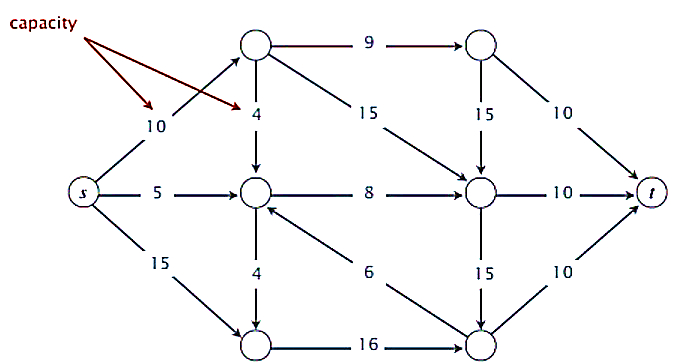
\includegraphics[width=0.65\textwidth]{figures/p3.jpg}}
}
	
%//////////////////////////////////////////////////////////////////////////////////////////////%%4
	\frame{
		\frametitle{A Cache Maintainence Problem}
	\begin{definition}
		A \ccp{cache} is a faster store device than memory which is used to reduce the times of access to memory.

		A \ccp{cache miss} is that when a data item \ccp{d} is requested, \ccp{d} is not in cache. 
	\end{definition}\pause

	\begin{definition}
		We have a set U of \ccp{n} pieces of data stored in main memory and 
		a cache which can hold \ccp{k (k<n)} items.
		Given a visiting sequence of data items \ccp{D ($d_1, d_2, d_3 ... d_m$)} from \ccp{U},
		\ccb{a eviction schedule} to determain which items should be evicted from the cache at which points 
		in the sequence. 
    \end{definition}\pause\bigskip

	}
	%%%//////////////////////////////////////////////////////////////////////////////////////////////%%5


	\frame{
	\frametitle{Cache Maintainence Problem}
	\begin{definition}
		We have a set U of \ccp{n} pieces of data stored in main memory and 
		a cache which can hold \ccp{k (k<n)} items.
		Given a visiting sequence of data items \ccp{D ($d_1, d_2, d_3 ... d_m$)} from \ccp{U},
		\ccb{a eviction schedule} to determain which items should be evicted from the cache at which points 
		in the sequence. 
	\end{definition}
	
	\centerline{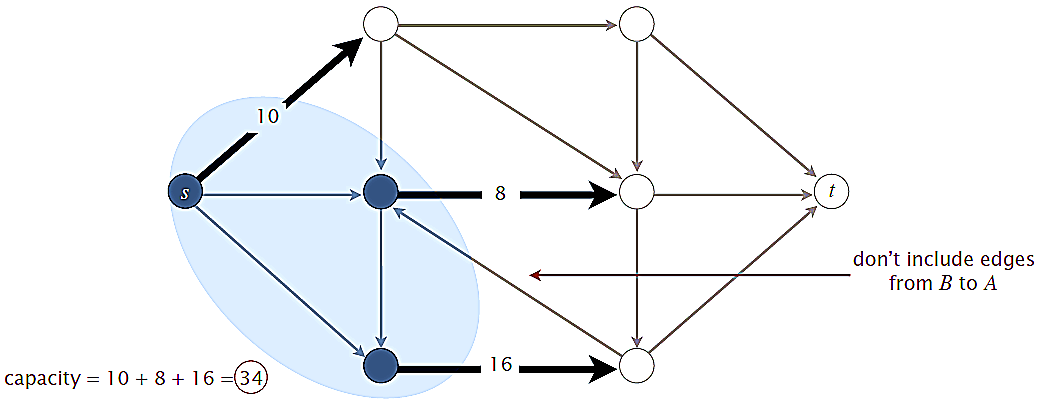
\includegraphics[width=0.7\textwidth]{figures/p5}}
}
	%%//////////////////////////////////////////////////////////////////////////////////////////////%%6

	\frame{
	\frametitle{Cache Maintainence Problem}
	
	\cco{Cache Maintainence Problem.} 
	Find an eviction schedule which makes the least number of cache misses.\bigskip\bigskip

	\centerline{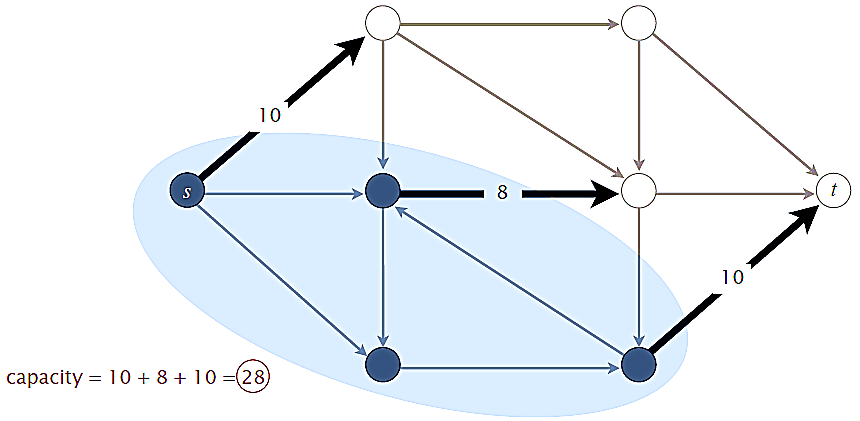
\includegraphics[width=0.6\textwidth]{figures/p6}}
}

	
%%//////////////////////////////////////////////////////////////////////////////////////////////%%7



		\frame{
		\frametitle{Quiz 1}
	Which is the capacity of the given $st$-cut?
\begin{enumerate}[\color{blue} A.]
	\item $11~ (20+25 - 8 - 11 - 9 - 6)$
	\item $34 ~(8+11+9+6)$
	\item $45~ (20+ 25)$
	\item $79~	(20+ 25+ 8+ 11+ 9+ 6)$
\end{enumerate}	
\vspace{5mm}
	
	\centerline{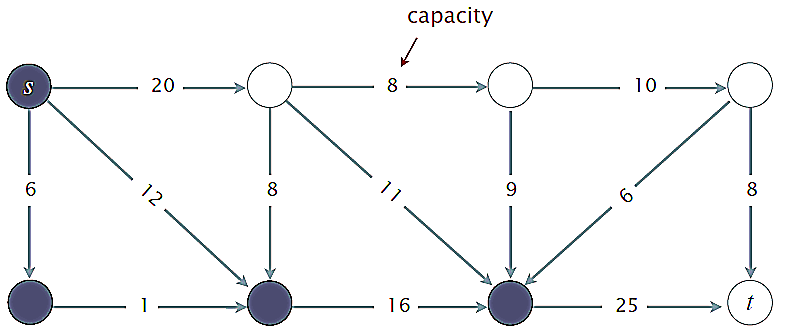
\includegraphics[width=0.8\textwidth]{figures/p7}}
	
}
	
	
	
	%%//////////////////////////////////////////////////////////////////////////////////////////////%%8
	\frame{
		\frametitle{Maximum-flow problem}
	\begin{definition}
		An \ccp{$st$-flow(flow)} \ccb{$f$} is a function that satisfies:
		\begin{itemize}
			\item For each \ccb{$e\in E$}: \hspace{2mm}  \ccb{$0 \leq f(e) \leq c(e)$}
			\item For each \ccb{$v\in V-\{s,t\}$}:  \ccb{$\sum\limits_{e \text { in to } v} f(e) \  =\sum\limits_{e \text { out of } v} f(e)$}
		\end{itemize}
	\end{definition}
	\bigskip

	\centerline{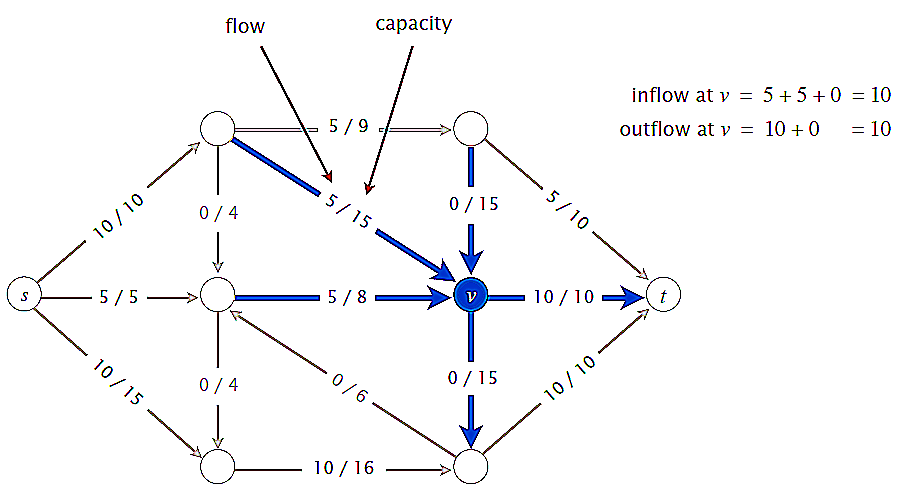
\includegraphics[width=0.8\textwidth]{figures/p8}}
	}
	
	%%//////////////////////////////////////////////////////////////////////////////////////////////%%9
	\frame{
		\frametitle{Maximum-flow problem}
		\begin{definition}
		An \ccp{$st$-flow(flow)} \ccb{$f$} is a function that satisfies:
		\begin{itemize}
			\item For each \ccb{$e\in E$}: \hspace{2mm}  \ccb{$0 \leq f(e) \leq c(e)$}
			\item For each \ccb{$v\in V-\{s,t\}$}:  \ccb{$\sum\limits_{e \text { in to } v} f(e) \  =\sum\limits_{e \text { out of } v} f(e)$}
		\end{itemize}
	\end{definition}
		\begin{definition}
		The \ccp{value}	of a flow \ccb{$f$} is: \ccb{$val(f)=\sum\limits_{e \text { out of } s} f(e)-\sum\limits_{e \text { in to } s} f(e)$}
		\end{definition}\smallskip
	
	\centerline{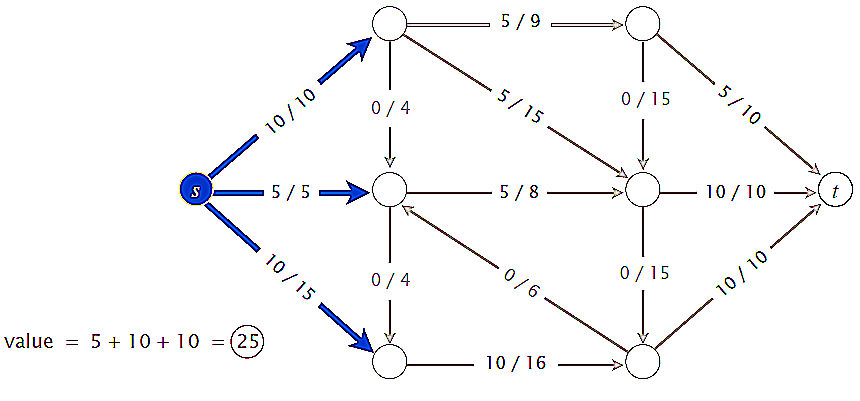
\includegraphics[width=0.7\textwidth]{figures/p9}}
	}
	
	
%%////////////////////////////////////////////////////////////////////////////////////////////%%10
	\frame{
	\frametitle{Maximum-flow problem}
	
    \cco{Max-flow problem.} Find a flow of maximum value.\bigskip\bigskip


	\centerline{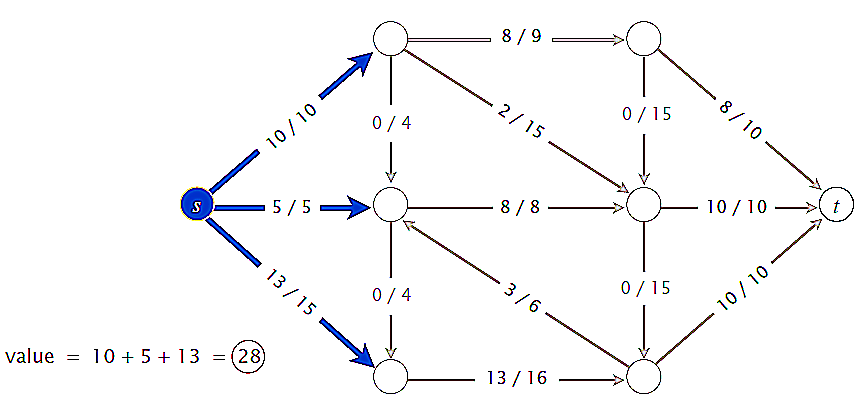
\includegraphics[width=0.7\textwidth]{figures/p10}}
}


\section{Ford-Fulkerson Algorithm}
	%
	%%//////////////////////////////////////////////////////////////////////////////////////////////%%12
	\frame{
		\frametitle{Toward a max-flow algorithm}
	\ccp{Greedy algorithm.}
	\vspace{-4mm}
		\begin{itemize}
			\item Start with \ccb{$f (e) = 0$} for each edge \ccb{$e \in E$}.
		\ccg{	\item Find an $s\rightsquigarrow t$ path $P$ where each edge has $f (e) < c(e)$.
			\item Augment flow along path $P$.
			\item  Repeat until you get stuck.}
		\end{itemize}\vspace{5mm}
	
	 	\centerline{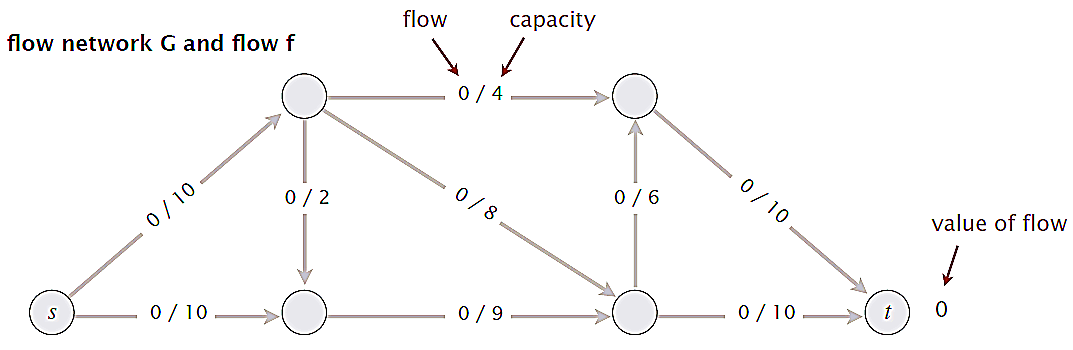
\includegraphics[width=\textwidth]{figures/p12}}
	}
	%
	%%//////////////////////////////////////////////////////////////////////////////////////////////%%13

\frame{
	\frametitle{Toward a max-flow algorithm}
	\ccp{Greedy algorithm.}
	\vspace{-4mm}
	\begin{itemize}
		\ccg{	\item Start with $f (e) = 0$ for each edge $e \in E$.}
		\item Find an \ccb{$s\rightsquigarrow t$} path \ccb{$P$} where each edge has \ccb{$f (e) < c(e)$}.
		\ccg{	\item Augment flow along path $P$.
			\item  Repeat until you get stuck.}
	\end{itemize}\vspace{5mm}
	
		\centerline{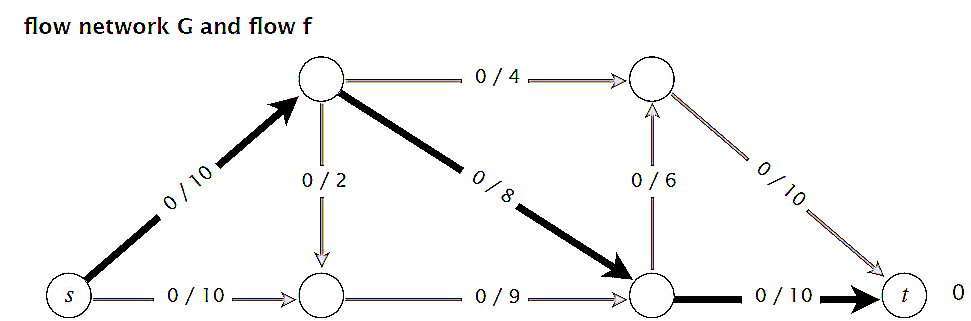
\includegraphics[width=\textwidth]{figures/p13}}
}
	%
	%%%%//////////////////////////////////////////////////////////////////////////////////////////////%%14
	%
\frame{
	\frametitle{Toward a max-flow algorithm}
	\ccp{Greedy algorithm.}
	\vspace{-4mm}
	\begin{itemize}
		\ccg{	\item Start with $f (e) = 0$ for each edge $e \in E$.
		\item Find an $s\rightsquigarrow t$ path $P$ where each edge has $f (e) < c(e)$.}
		\item Augment flow along path \ccb{$P$}.
		\ccg{	\item  Repeat until you get stuck.}
	\end{itemize}\vspace{5mm}
	
		\centerline{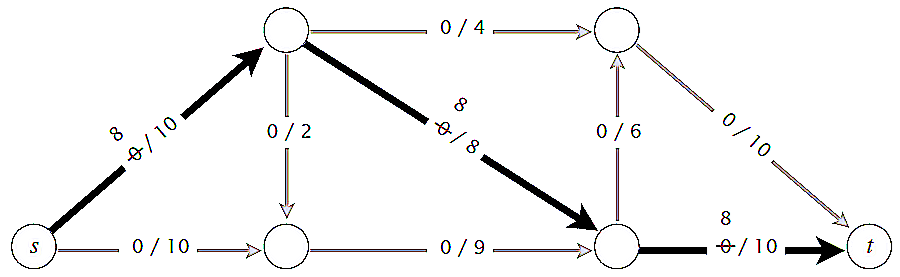
\includegraphics[width=\textwidth]{figures/p14}}
}
	%%%//////////////////////////////////////////////////////////////////////////////////////////////%%15
	
\frame{
	\frametitle{Toward a max-flow algorithm}
	\ccp{Greedy algorithm.}
	\vspace{-4mm}
	\begin{itemize}
		\ccg{	\item Start with $f (e) = 0$ for each edge $e \in E$.
			\item Find an $s\rightsquigarrow t$ path $P$ where each edge has $f (e) < c(e)$.
		\item Augment flow along path $P$.}
			\item  Repeat until you get stuck.
	\end{itemize}\vspace{3mm}
	
		\centerline{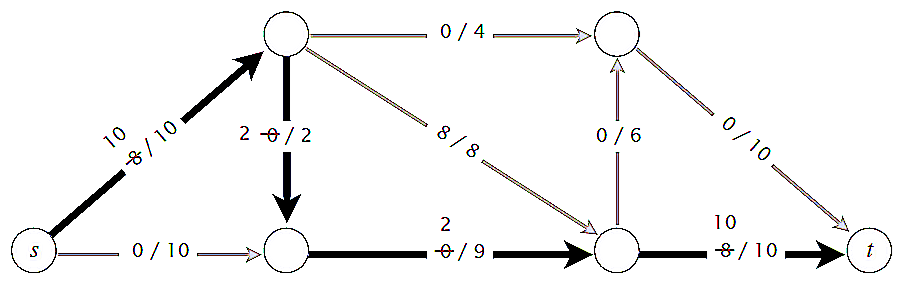
\includegraphics[width=\textwidth]{figures/p15}}
}
	%%%%//////////////////////////////////////////////////////////////////////////////////////////////%%16
   \frame{
	\frametitle{Toward a max-flow algorithm}
	\ccp{Greedy algorithm.}
	\vspace{-4mm}
	\begin{itemize}
		\ccg{\item Start with $f (e) = 0$ for each edge $e \in E$.
			\item Find an $s\rightsquigarrow t$ path $P$ where each edge has $f (e) < c(e)$.
			\item Augment flow along path $P$.}
		\item  Repeat until you get stuck.
	\end{itemize}\vspace{5mm}

	
		\centerline{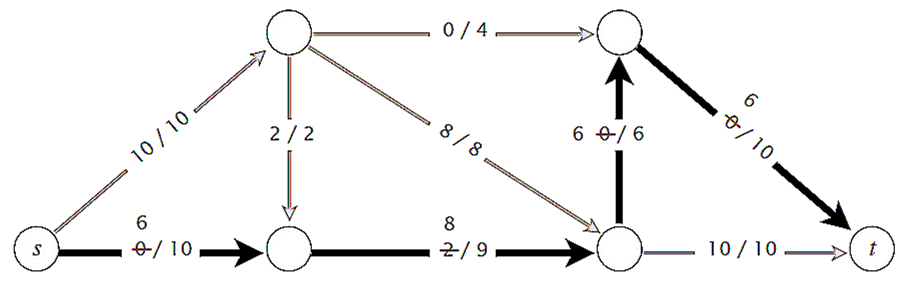
\includegraphics[width=\textwidth]{figures/p16}}
}
	%%%%//////////////////////////////////////////////////////////////////////////////////////////////%%17
\frame{
	\frametitle{Toward a max-flow algorithm}
	\ccp{Greedy algorithm.}
	\vspace{-4mm}
	\begin{itemize}
			\item Start with \ccb{$f (e) = 0$} for each edge \ccb{$e \in E$}.
			\item Find an \ccb{$s\rightsquigarrow t$} path \ccb{$P$} where each edge has \ccb{$f (e) < c(e)$}.
			\item Augment flow along path \ccb{$P$}.
		\item  Repeat until you get stuck.
	\end{itemize}
\bigskip

	
		\centerline{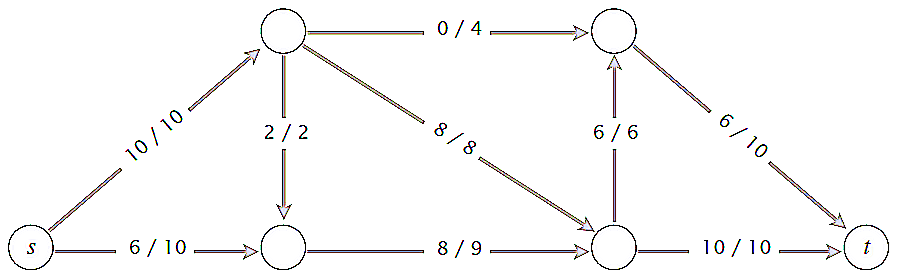
\includegraphics[width=\textwidth]{figures/p17}}
}
%%%%//////////////////////////////////////////////////////////////////////////////////////////////%%18

  \frame{
	\frametitle{Toward a max-flow algorithm}
	\ccp{Greedy algorithm.}
	\vspace{-4mm}
	\begin{itemize}
			\item Start with \ccb{$f (e) = 0$} for each edge \ccb{$e \in E$}.
			\item Find an \ccb{$s\rightsquigarrow t$} path \ccb{$P$} where each edge has \ccb{$f (e) < c(e)$}.
			\item Augment flow along path \ccb{$P$}.
		\item  Repeat until you get stuck.
	\end{itemize}
\bigskip
	
		\centerline{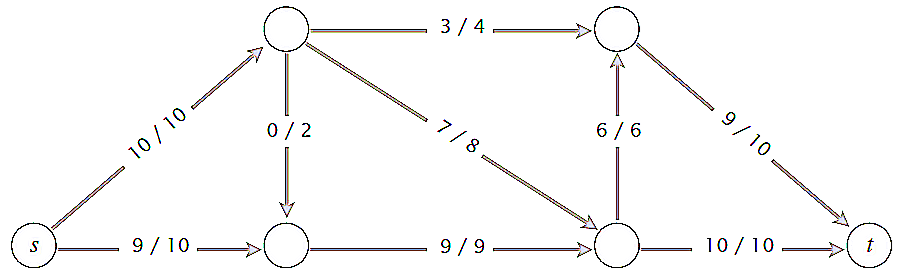
\includegraphics[width=\textwidth]{figures/p18}}
}
	
%%%%//////////////////////////////////////////////////////////////////////////////////////////////%%19

	\frame{
    \frametitle{Why the greedy algorithm fails}
		\ccr{Q.} Why does the greedy algorithm fail?\pause

		\ccc{A.} Once greedy algorithm increases flow on an edge, it never decreases it.
		\pause\smallskip
		
		\cco{Ex.} Consider flow network \ccb{$G$}.	\vspace{-3mm}
		\begin{itemize}
			\item The unique max flow has \ccb{$f^*(v,w)=0$}.
			\item Greedy algorithm could choose \ccb{$s\rightarrow v\rightarrow w \rightarrow t$} as first augmenting path.
		\end{itemize}\smallskip
		
		\centerline{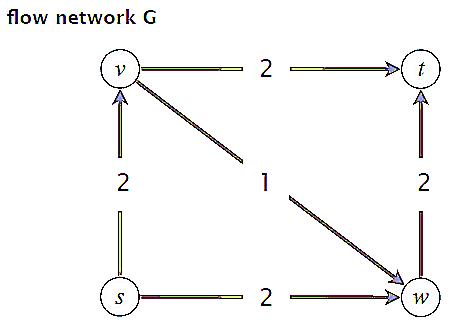
\includegraphics[width=0.4\textwidth]{figures/p19}}\pause
		
	\cco{Bottom line.} Need some mechanism to \ccr{undo} a bad decision.	
	}
	%%%%//////////////////////////////////////////////////////////////////////////////////////////////%%20
	\frame{
		\frametitle{Residual network}
		\vspace{2mm}
	\begin{columns}
		\begin{column}{6cm}
			\ccp{Original edge} \ccb{$e=(u,v)\in E$}.
			\begin{itemize}
				\item Flow \ccb{$f(e)$}.
				\item Capacity \ccb{$c(e)$}
			\end{itemize}	
		\vspace{3mm}
		
			\ccp{Reverse edge}  \ccb{$e^{\text { reverse }}=(v, u)$}
			\begin{itemize}
				\item	\cco{Undo} flow sent.
			\end{itemize}	
		
		\end{column}
	
		\begin{column}{4cm}
	\centerline{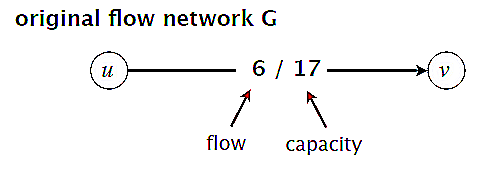
\includegraphics[width=\textwidth]{figures/p20}}
	\end{column}
	\end{columns}
\bigskip\pause
	\begin{columns}
		
	\begin{column}{6cm}
\ccp{Residual capacity}
\ccb{$$
c_{f}(e)=\left\{\begin{array}{ll}{c(e)-f(e)} & {\text { if } e \in E} \\ {f(e)} & {\text { if } e^{\text { reverse }} \in E}\end{array}\right.
$$}
  \end{column}
	
	\begin{column}{4cm}
		\centerline{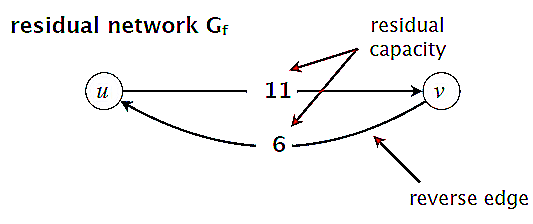
\includegraphics[width=\textwidth]{figures/p20_2}}
	\end{column}
\end{columns}


\ccp{Residual network} \ccb{$G_f=(V,E_f,s,t,c_f)$} 	%$ \color{red}\begin{array}{l}
%\text{\tiny edges with positive}\\[-2mm]
%\text{\tiny residual capacity}\\
%\swarrow\\
%\end{array} $ 	\vspace{-4mm}
\begin{itemize}
		\vspace{-4mm}
	\item \ccb{$E_{f}=\{e : f(e)<c(e)\} \cup\left\{e^{\text { reverse }} : f(e)>0\right\}$}.	%$ \color{red}\begin{array}{l}
%	\text{\tiny where flow on a reverse edge}\\[-2mm]
% \quad	\text{\tiny negates flow on}\\[-2mm]
%	\text{\tiny corresponding forward edge}\\
%	\swarrow\\
%	\end{array} $
% \vspace{-2mm}
	\item Key property: \ccb{$f'$} is a flow in \ccb{$G_f$} iff \ccb{$f+f'$} is a flow in \ccb{$G$}
\end{itemize}
	}
	%%
%%%%//////////////////////////////////////////////////////////////////////////////////////////////%%21

\frame{
	\frametitle{Augmenting path}
	\begin{definition}
		An \ccp{augmenting path} is a simple \ccb{$s\rightsquigarrow t$} path in the residual network \ccb{$G_f$}.
	\end{definition}\pause

  \begin{definition}
	The \ccp{bottleneck capacity} of an augmenting path \ccb{$P$} is the minimum residual capacity of any edge in \ccb{$P$}.	
   \end{definition}
  }

%%%%//////////////////////////////////////////////////////////////////////////////////////////////%%21

\frame{
	\frametitle{Augmenting path}

    \cco{Key Property.}
    Let \ccb{$f$} be a flow and let \ccb{$P$} be an augmenting path in \ccb{$G_f$}. After calling \ccb{$f'\leftarrow\mathtt{Augment}(f,c,P)$}, the resulting \ccb{$f'$} is a flow and \ccb{$val(f')=val( f )+bottleneck(G_f, P)$}.\pause

    \begin{exampleblock}{}
   % \scalebox{0.9}{
    \begin{algorithm}[H]
        \SetKwData{x}{x}\SetKwData{y}{y}\SetKwData{z}{z}
        \SetKwFunction{Au}{\sc Augment}\SetKwFunction{Return}{\sc Return}\SetKwFunction{Init}{\sc Initialize}
        \SetKwInOut{Input}{input}\SetKwInOut{Output}{output}
     \Au{$f$,$c$,$P$}
     \BlankLine
     $\delta \leftarrow$ bottleneck capacity of augmenting path P\;
     \For{each edge $e\in P$}{
       \lIf{$(e\in E)$}{$f(e)\leftarrow f(e)+\delta$}
      \Else{$f\left(e^{\text { reverse }}\right) \leftarrow f\left(e^{\text { reverse }}\right)-\delta$}
      }
      \Return $f$\;
     \end{algorithm}
     \end{exampleblock}

     }
	%%
	%%%%//////////////////////////////////////////////////////////////////////////////////////////////%%22
	%
	\frame{
		\frametitle{Network flow: quiz 2}
	Which is the augmenting path of highest bottleneck capacity?
	\begin{enumerate}\color{blue}
		\item $A \rightarrow F \rightarrow G \rightarrow H$
		\item $A \rightarrow B \rightarrow C \rightarrow D \rightarrow H$
		\item $A \rightarrow F \rightarrow B \rightarrow G \rightarrow H$
		\item $A \rightarrow F \rightarrow B \rightarrow G \rightarrow C \rightarrow D \rightarrow H$
	\end{enumerate}	\vspace{3mm}
		\centerline{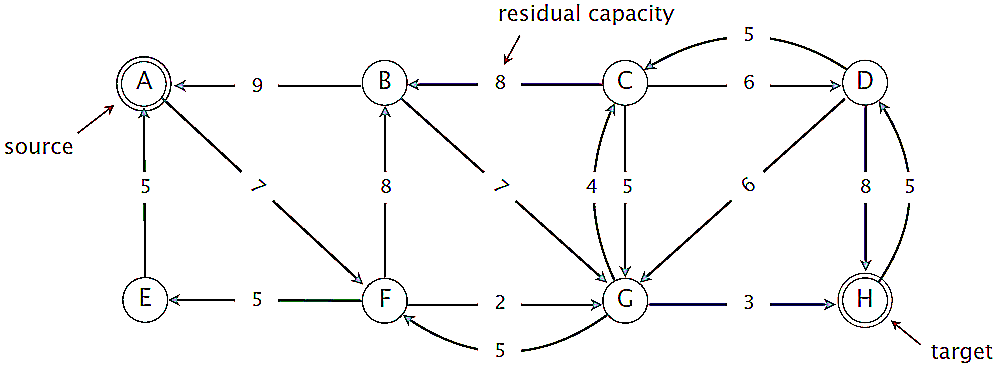
\includegraphics[width=0.8\textwidth]{figures/p22}}
	}
	%%
	%%%%//////////////////////////////////////////////////////////////////////////////////////////////%%23
	\frame{
		\frametitle{Ford–Fulkerson algorithm}
		\ccp{Ford–Fulkerson augmenting path algorithm.}
		\vspace{-3mm}
		\begin{itemize}
		\item Start with \ccb{$f (e) = 0$} for each edge \ccb{$e \in E$}.
		\item Find an \ccb{$s\rightsquigarrow t$} path \ccb{$P$}  in the residual network \ccb{$G_f$}.
		\item Augment flow along path \ccb{$P$}.
		\item  Repeat until you get stuck.
		\end{itemize}
	\pause

	\begin{exampleblock}{}
    \begin{algorithm}[H]
        \SetKwData{x}{x}\SetKwData{y}{y}\SetKwData{z}{z}
        \SetKwFunction{FF}{\sc Ford–Fulkerson}\SetKwFunction{Return}{\sc Return}\SetKwFunction{Init}{\sc Initialize}
        \SetKwFunction{Up}{\sc Update}\SetKwFunction{Au}{\sc Augment}
        \SetKwInOut{Input}{input}\SetKwInOut{Output}{output}
     \FF{$G$}
     \BlankLine
     \For{each edge $e \in E$}{$f(e)\leftarrow 0$}
     $G_f\leftarrow $ residual network of $G$ with respect to flow $f$\;

     \While{there exists an $s\rightsquigarrow t$ path $P$ in $G_f$}{
      $f\leftarrow$ \Au{$f$,$c$,$P$}\;
      \Up{$G_f$}\;
      }
      \Return $f$\;
     \end{algorithm}
     \end{exampleblock}

	}
	%%%%//////////////////////////////////////////////////////////////////////////////////////////////%%24

	\section{Max-Flow Min-Cut Theorem}

	%%%%//////////////////////////////////////////////////////////////////////////////////////////////%%25
	
	\frame{
		\frametitle{Relationship between flows and cuts}
		\begin{lemma}
		Let \ccb{$f$} be any flow and let \ccb{$(A,B)$} be any cut. Then, the value of the flow \ccb{$f$} equals the net flow across the cut \ccb{$(A,B)$}.	
		\ccb{\begin{equation*}
	v a l(f)=\sum\limits_{\text { out of } A} f(e)-\sum\limits_{e \text { in to } A} f(e)
		\end{equation*}}
    \end{lemma}
	
	\bigskip
   \centerline{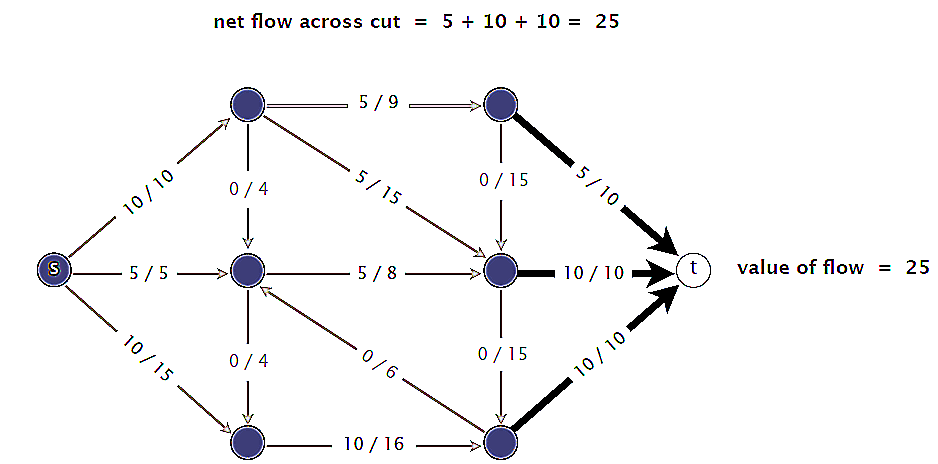
\includegraphics[width=0.8\textwidth]{figures/p25}}
	}
	%
	%%%%//////////////////////////////////////////////////////////////////////////////////////////////%%26
	\frame{
	\frametitle{Relationship between flows and cuts}
		\begin{lemma}
		Let \ccb{$f$} be any flow and let \ccb{$(A,B)$} be any cut. Then, the value of the flow
     \ccb{$f$} equals the net flow across the cut \ccb{$(A,B)$}.	
		\ccb{\begin{equation*}
	v a l(f)=\sum\limits_{\text { out of } A} f(e)-\sum\limits_{e \text { in to } A} f(e)
		\end{equation*}}
    \end{lemma}
	
	\bigskip
\centerline{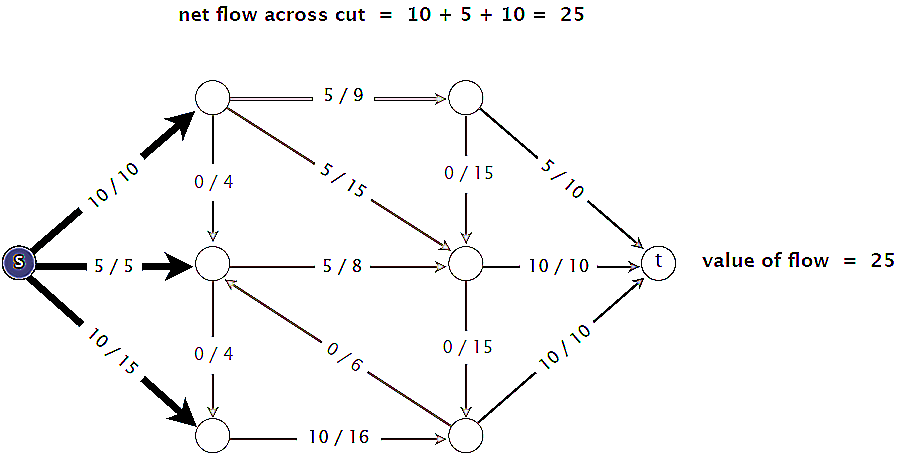
\includegraphics[width=0.8\textwidth]{figures/p26}}
}
	%
	%%%//////////////////////////////////////////////////////////////////////////////////////////////%%27
	
			\frame{
		\frametitle{Relationship between flows and cuts}
	\begin{lemma}
		Let \ccb{$f$} be any flow and let \ccb{$(A,B)$} be any cut. Then, the value of the flow
     \ccb{$f$} equals the net flow across the cut \ccb{$(A,B)$}.	
		\ccb{\begin{equation*}
	v a l(f)=\sum\limits_{\text { out of } A} f(e)-\sum\limits_{e \text { in to } A} f(e)
		\end{equation*}}
    \end{lemma}
	
	\bigskip
    \centerline{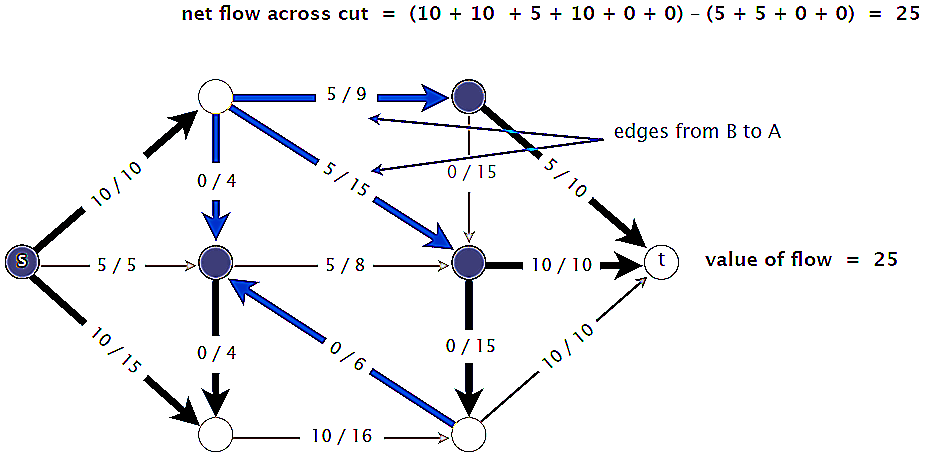
\includegraphics[width=0.8\textwidth]{figures/p27}}
	}
	%%%%//////////////////////////////////////////////////////////////////////////////////////////////%%28
	\frame{
	\frametitle{Network flow: quiz 3}	
	Which is the net flow across the given cut?
	\begin{enumerate}\color{blue}
		\item 11 $ (20+25- 8- 11- 9- 6) $
		\item 26 $ (20+22- 8- 4- 4) $
		\item  42 $ (20+22) $
		\item 45 $ (20+25) $
	\end{enumerate}
	\bigskip
 \centerline{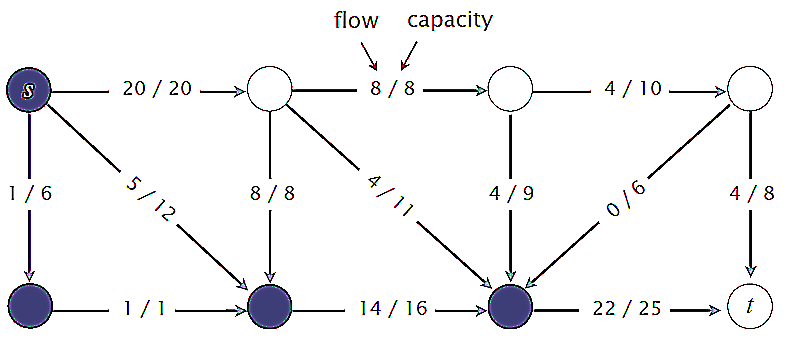
\includegraphics[width=0.8\textwidth]{figures/p28}}
}



	%%%%//////////////////////////////////////////////////////////////////////////////////////////////%%29
		\frame{
		\frametitle{Relationship between flows and cuts}
	\begin{lemma}
		Let \ccb{$f$} be any flow and let \ccb{$(A,B)$} be any cut. Then, the value of the flow
     \ccb{$f$} equals the net flow across the cut \ccb{$(A,B)$}.	
		\ccb{\begin{equation*}
	v a l(f)=\sum\limits_{\text { out of } A} f(e)-\sum\limits_{e \text { in to } A} f(e)
		\end{equation*}}
    \end{lemma}\pause

\ccm{\em Proof.}

\ccb{$$\begin{array}{ll}
val(f)&=\sum\limits_{e \text { out of } s} f(e)-\sum\limits_{\text { e in to } s} f(e) \\
&=\sum\limits_{v \in A}\left(\sum\limits_{e \text { out of } v} f(e)-\sum\limits_{\text { e in to } v} f(e)\right)\\
&=\sum\limits_{e \text { out of } A} f(e)-\sum\limits_{e \text { in to } A} f(e).
\end{array}
$$}


}

	%%//////////////////////////////////////////////////////////////////////////////////////////////%%30
	\frame{
		\frametitle{Relationship between flows and cuts}
		\begin{theorem}{Weak Duality}
         Let \ccb{$f$} be any flow and \ccb{$(A, B)$} be any cut. Then, \ccb{$val(f) \leq \operatorname{cap}(A, B)$}.
         \end{theorem}\pause
	
\ccm{\em Proof.}
\ccb{	
$$
\begin{aligned}
\operatorname{val}(f) &=\sum_{e \text { out of } A} f(e)-\sum_{\text {e  in to } A} f(e) \\
& \leq \sum_{\text { e out of } A} f(e) \\
& \leq \sum_{e \text { out of } A} c(e) \\
&=\operatorname{cap}(A, B)
 \end{aligned}
$$}
		\vspace{3mm}\centerline{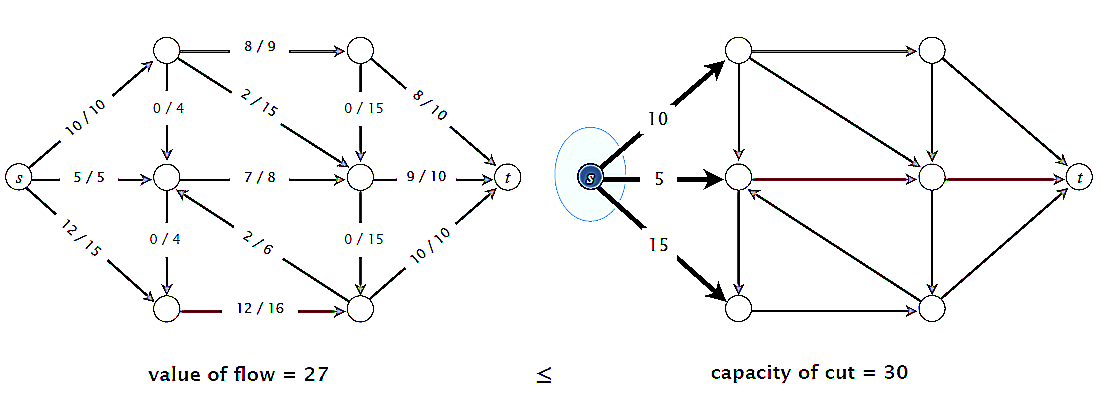
\includegraphics[width=0.8\textwidth]{figures/p30}}
	}
	%%
	%%
	%%%%//////////////////////////////////////////////////////////////////////////////////////////////%%31
	%
	\frame{
		\frametitle{Certificate of optimality}
	\begin{corollary}
		Let \ccb{$f$} be a flow and let \ccb{$(A,B)$} be any cut.
		If \ccb{$val(f)=\operatorname{cap}(A, B)$}, then \ccb{$f$} is a max flow and \ccb{$(A,B)$} is a min cut.
	\end{corollary}\pause
	
	\ccm{\em Proof.}\vspace{-2mm}
%\hspace{3.5cm}	$ \color{red}\begin{array}{l}	
%		\text{\tiny weak duality}\\[-1mm]
%			\swarrow
%	\end{array} $
	\begin{itemize}
		\vspace{-3mm}
		\item For any flow \ccb{$f^{\prime} : \quad {val}\left(f^{\prime}\right) \leq 	\operatorname{cap}(A, B)=val(f)$}.
		\item For any cut \ccb{$\left(A^{\prime}, B^{\prime}\right) : \operatorname{cap}\left(A^{\prime}, B^{\prime}\right) \geq {val}(f)=\operatorname{cap}(A, B)$}
	\end{itemize}	
%\vspace{-3mm}
%\hspace{5.5cm}	$ \color{red}\begin{array}{l}	
%\nwarrow\\[-2mm]
%	\text{\tiny weak duality}
%	\end{array} $
	
		\vspace{3mm}\centerline{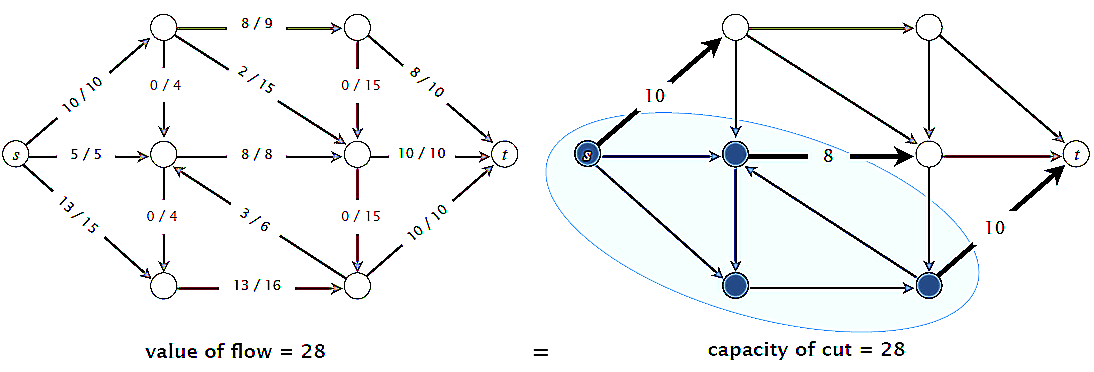
\includegraphics[width=0.8\textwidth]{figures/p31}}
	
	}
	%
	%%%%//////////////////////////////////////////////////////////////////////////////////////////////%%32
	%
	\frame{
		\frametitle{Max-flow min-cut theorem}

	\begin{block}{Max-Flow Min-Cut Theorem}	Value of a max flow = capacity of a min cut.
     \end{block}
		
	\vspace{6mm}\centerline{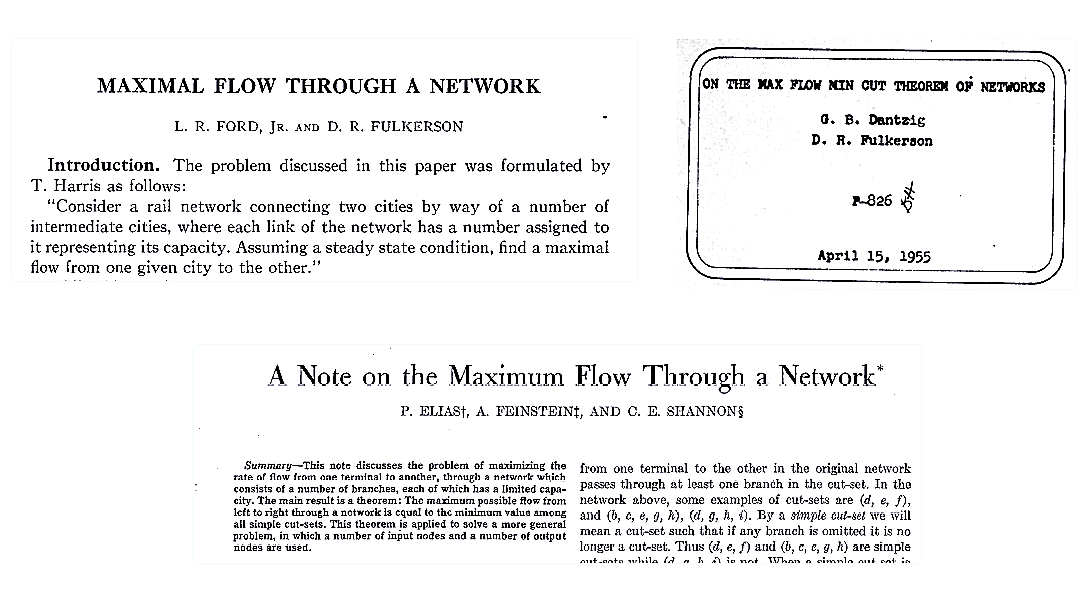
\includegraphics[width=\textwidth]{figures/p32}}
	}
	%%
	%
	%%%%//////////////////////////////////////////////////////////////////////////////////////////////%%33
		\frame{
		\frametitle{Max-flow min-cut theorem}
		\begin{block}{Max-Flow Min-Cut Theorem}	Value of a max flow = capacity of a min cut.
     \end{block}\pause

		\begin{block}{Augmenting path theorem} A flow \ccb{$f$} is a max flow iff no augmenting paths.
        \end{block}\pause
        	
		\ccm{\em Proof.}  The following three conditions are equivalent for any flow \ccb{$f$}:\vspace{-3mm}\pause
		\begin{enumerate}[i.]
			\item There exists a cut \ccb{$(A, B)$} such that \ccb{$\operatorname{cap}(A, B)=val(f)$}.
			\item  \ccb{$f$} is a max flow.
			\item  There is no augmenting path with respect to \ccb{$f$}.
%$	 \color{red}\leftarrow\begin{array}{l}
%			\text{\tiny if Ford–Fulkerson terminates,}\\[-2mm]
%			\quad\text{\tiny (then $f$ is max flow)}
%			\end{array} $
		\end{enumerate}\pause

		\ccc{[i$\Rightarrow$ ii]}\pause \hspace{2em}	This is the weak duality corollary.
			
	}
	
	%%%%//////////////////////////////////////////////////////////////////////////////////////////////%%34
	\frame{
	\frametitle{Max-flow min-cut theorem}
		\begin{block}{Max-Flow Min-Cut Theorem}	Value of a max flow = capacity of a min cut.
     \end{block}
		\begin{block}{Augmenting path theorem} A flow \ccb{$f$} is a max flow iff no augmenting paths.
        \end{block}
        	
		\ccm{\em Proof.}  The following three conditions are equivalent for any flow \ccb{$f$}:\vspace{-3mm}
		\begin{enumerate}[i.]
			\item There exists a cut \ccb{$(A, B)$} such that \ccb{$\operatorname{cap}(A, B)=val(f)$}.
			\item  \ccb{$f$} is a max flow.
			\item  There is no augmenting path with respect to \ccb{$f$}.
%$	 \color{red}\leftarrow\begin{array}{l}
%			\text{\tiny if Ford–Fulkerson terminates,}\\[-2mm]
%			\quad\text{\tiny (then $f$ is max flow)}
%			\end{array} $
		\end{enumerate}

	\ccc{[ii$\Rightarrow$ iii]}	 \pause\hspace{2em} We prove contrapositive: \ccov{$\lnot$ iii $\Rightarrow \lnot $ii}.\\ \pause
	\begin{itemize}
		\item  Suppose that there is an augmenting path with respect to \ccb{$f$}.
		\item Can improve flow \ccb{$f$} by sending flow along this path.
		\item Thus, \ccb{$f$} is not a max flow.
	\end{itemize}
	
	
}
	%
	%%%%//////////////////////////////////////////////////////////////////////////////////////////////%%35
	\frame{
		\frametitle{Max-flow min-cut theorem}
		\ccc{[ iii $\Rightarrow$ i ]}\vspace{-1em}
		\begin{itemize}
			\item Let \ccb{$f$} be a flow with no augmenting paths.
			\item Let \ccb{$A$} be set of nodes reachable from \ccb{$s$} in residual network \ccb{$G_f$}.
			\item By definition of \ccb{$A: s \in A$}.
			\item By definition of flow \ccb{$f: t \notin A$}.
		\end{itemize}
		
		\begin{columns}
			\begin{column}{6cm}
			\ccb{$$
			\begin{aligned}
			{val}(f) &=\sum_{e \text { out of } A} f(e)-\sum_{\text {e  in to } A} f(e) \\
			%\color{red}\begin{array}{l}
%			\hspace{5mm}\nearrow\\
%			\text{\tiny flow value}\\[-2mm]
%			\hspace{2mm}\text{\tiny lemma}
%			\end{array}
          & = \sum_{\text { e out of } A} c(e)  -  0 \\
			&=\operatorname{cap}(A, B)
			\end{aligned}
			$$}
			\end{column}
		\begin{column}{6cm}
				\vspace{3mm}\centerline{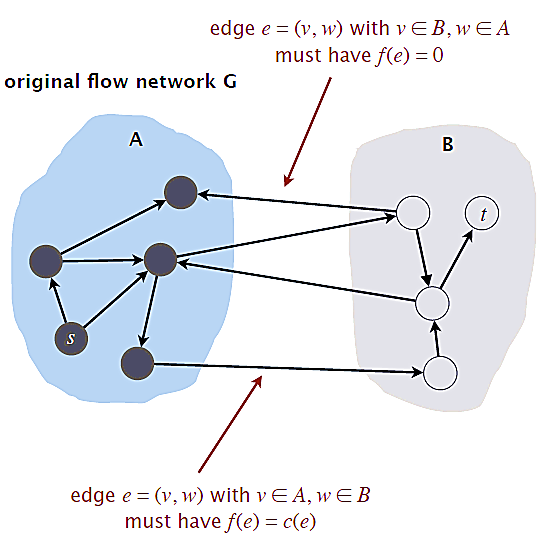
\includegraphics[width=0.8\textwidth]{figures/p35}}     			
		\end{column}
		\end{columns}
	}

%%//////////////////////////////////////////////////////////////////////////////////////////////%%36
	
    \section{Capacity-Scaling Algorithm}
	
%%//////////////////////////////////////////////////////////////////////////////////////////////%%37
	%%
	%%
	\frame{
		\frametitle{Analysis of Ford–Fulkerson algorithm (when capacities are integral)}

		\ccp{Assumption.} Every edge capacity \ccb{$c(e)$} is an integer between \ccb{$1$} and \ccb{$C$}.\pause
		
		\ccp{Integrality invariant.} Throughout Ford-Fulkerson, every edge flow \ccb{$f(e)$} and residual capacity \ccb{$c_f (e)$} is an integer.\pause

		\ccm{\em Proof.}  By induction on the number of augmenting paths.\pause

%%	\vspace{-2mm}	
%			
%	\hspace{6cm}	$ \color{red}\begin{array}{l}	
%		\quad\text{\tiny  consider cut A =\{ s \}}\\[-2mm]
%		\text{\tiny (assumes no parallel edges)
%			}\\[-2mm]
%	\hspace{1cm} \swarrow
%		\end{array} $\vspace{-7mm}

		\begin{theorem}
		Ford–Fulkerson terminates after at most \ccb{$val\left(f^{*}\right) \leq n C$}\\
		augmenting paths, where \ccb{$f^*$} is a max flow.
		\end{theorem}\pause

	\ccm{\em Proof.} Each augmentation increases the value of the flow by at least 1.
	
	}

%%//////////////////////////////////////////////////////////////////////////////////////////////%%37

	\frame{
		\frametitle{Analysis of Ford–Fulkerson algorithm (when capacities are integral)}
    \begin{corollary}
	The running time of Ford–Fulkerson is \ccb{$O(m n C)$}.
		\end{corollary}	\pause

   \ccm{\em Proof.} Can use either BFS or DFS to find an augmenting path in \ccb{$O(m)$} time.\pause
	
%\hspace{4cm}	$ \color{red}\begin{array}{l}
%	\quad\text{\tiny $f (e)$ is an integer for every $e$}\\
%\hspace{1.5cm}\swarrow
%	\end{array} $
%	\vspace{-2mm}
	
	\begin{block}{Integrality Theorem} There exists an integral max flow \ccb{$f^*$}
    \end{block}\pause

	\ccm{\em Proof.}
     Since Ford–Fulkerson terminates, theorem follows from integrality invariant.

	}
	%%
	%%%%//////////////////////////////////////////////////////////////////////////////////////////////%%38
	
	\frame{
		\frametitle{Ford–Fulkerson: exponential example}
	\ccr{Q.} Is generic Ford–Fulkerson algorithm poly-time in input size?\pause
%	\hspace{6.8cm}\ccr{ $ \begin{array}{l}
%		\qquad\nearrow\\[-2mm]
%		\tiny\text{$ m,n $ and $ \log C $}
%		\end{array} $}	
%		\vspace{-3mm}
		
      \ccc{A.} No. If max capacity is \ccb{$C$}, then algorithm can take \ccb{$\geq C$} iterations.\pause

      \bigskip

      \begin{columns}
      	\begin{column}{4cm}
            \begin{itemize}\color{blue}
      	\item $s \rightarrow v \rightarrow w \rightarrow t$\
      	\item $s \rightarrow w \rightarrow v \rightarrow t$
      	\item $s \rightarrow v \rightarrow w \rightarrow t$
      	\item $s \rightarrow w \rightarrow v \rightarrow t$
      	\item $\dots$
      	\item $s \rightarrow v \rightarrow w \rightarrow t$
      	\item $s \rightarrow w \rightarrow v \rightarrow t$
      \end{itemize}
      		
      	\end{column}
      	\begin{column}{6cm}
      	\centerline{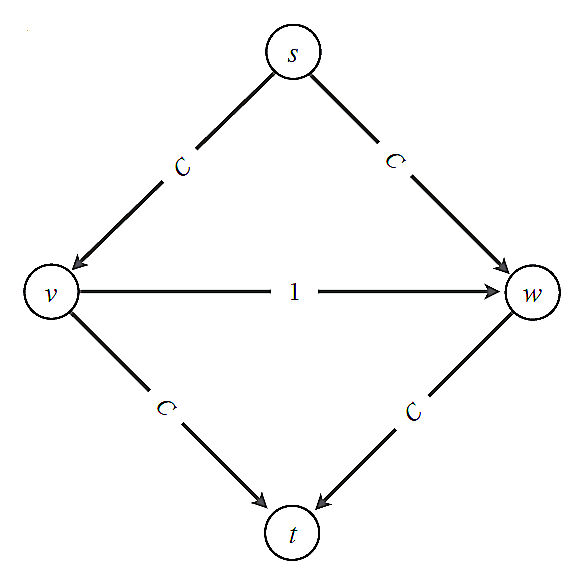
\includegraphics[width=\textwidth]{figures/p38}}
      	\end{column}
      \end{columns}
	}

	%%%%//////////////////////////////////////////////////////////////////////////////////////////////%%39

	\frame{
		\frametitle{Network flow: quiz 4}
		The Ford–Fulkerson algorithm is guaranteed to terminate if the edge capacities are $\ldots$
	\begin{enumerate}[A.]
		\item Rational numbers.
		\item Real numbers.
		\item Both A and B.
		\item Neither A nor B.
	\end{enumerate}
	}
	%%%%//////////////////////////////////////////////////////////////////////////////////////////////%%40
	
	\frame{
		\frametitle{Choosing good augmenting paths}
	\ccp{Use care when selecting augmenting paths.}	\vspace{-3mm}
	\begin{itemize}
		\item Some choices lead to exponential algorithms.
		\item Clever choices lead to polynomial algorithms.
	\end{itemize}\pause\bigskip

\ccp{Pathology.} When edge capacities can be irrational, no guarantee that Ford–Fulkerson terminates (or converges to a maximum flow)!
\pause\bigskip
		
\cco{Goal.}	Choose augmenting paths so that:\vspace{-3mm}
\begin{itemize}
	\item Can find augmenting paths efficiently.
	\item Few iterations.
\end{itemize}
		
	}
	
		%%%%//////////////////////////////////////////////////////////////////////////////////////////////%%41
	
    \frame{
	 \frametitle{Capacity-scaling algorithm: analysis of running time}

    \begin{block}{Lemma 2}
    There are \ccb{$\leq 2m$} augmentations per scaling phase.
    \end{block}\pause

    \ccm{\em Proof.} %\hspace{7cm}\ccr{ $ \begin{array}{l}
%	\quad\tiny\text{or equivalently}\\[-2mm]
%	\quad~\tiny\text{at the end}\\[-2mm]
%	\tiny\text{of a 2$\Delta$-scaling phase}\\
%	\qquad\swarrow\\
%	\end{array} $}\vspace{-6mm}
    \begin{itemize}
	\item Let \ccb{$f$} be the flow at the beginning of a $\Delta$-scaling phase.
	\item Lemma 3 \ccc{$\Rightarrow$} max-flow value  \ccb{$\leq {val}(f)+m(2 \Delta)$}.
	\item Each augmentation in a $\Delta$-phase increases \ccb{$val(f)$} by at least \ccb{$\Delta$}.
	
\end{itemize}
	
	}
%%%%//////////////////////////////////////////////////////////////////////////////////////////////%%46
	
	\frame{
		\frametitle{Capacity-scaling algorithm: analysis of running time}
    \begin{block}{Lemma 3}
	Let \ccb{$f$} be the flow at the end of a \ccb{$\Delta$}-scaling phase.\\
	Then, the max-flow value \ccb{$\leq \operatorname{val}(f)+m \Delta$}.
\end{block}\pause

    \ccm{\em Proof.} \vspace{-4mm}\pause
		\begin{itemize}
			\item We show there exists a cut \ccb{$(A, B)$} such that \ccb{$cap(A, B)\leq val(f) + m \Delta$}.
			\item Choose \ccb{$A$} to be the set of nodes reachable from \ccb{$s$} in \ccb{$G_f (\Delta)$}.
			\item By definition of \ccb{$A: s \in A$}.
			\item By definition of flow \ccb{$f: t \notin A$}.
		\end{itemize}
	\bigskip\pause

	\begin{columns}
	\hspace{2mm}	\begin{column}{6cm}
	\ccb{$\begin{array}{ll}
	val(f)&=\sum\limits_{e \text { out of } A} f(e)-\sum\limits_{e \text { in to } A} f(e)\\
	%\ccr{ \begin{array}{l}
%			~~\nearrow\\[-2mm]
%			\tiny\text{flow}\\[-2mm]
%			\tiny\text{value}\\[-2mm]			
%			\tiny\text{lemma}
%		\end{array} }
	  &\geq \sum\limits_{e \text { out of } A}(c(e)-\Delta)-\sum\limits_{\text { e in to } A} \Delta\\
	  &\geq \sum\limits_{e \text { out of } A} c(e)-\sum\limits_{e \text { out of } A} \Delta-\sum\limits_{e \text { in to } A} \Delta \\
	   &\geq \operatorname{cap}(A, B)-m \Delta
	   \end{array}$}
		\end{column}
	
	\begin{column}{5cm}
	\vspace{3mm}\centerline{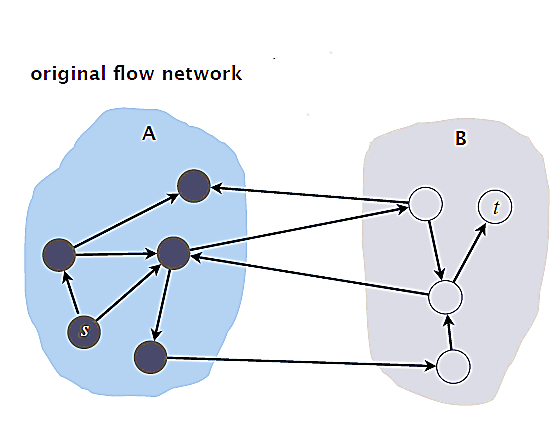
\includegraphics[width=0.8\textwidth]{figures/p46}}
	\end{column}
	\end{columns}	
		
	}

%%%%//////////////////////////////////////////////////////////////////////////////////////////////%%45

	\section{Shortest Augmenting Paths}

%%%%//////////////////////////////////////////////////////////////////////////////////////////////%%48
	%%
	\frame{
		\frametitle{Shortest augmenting path}
		\ccr{Q.} How to choose next augmenting path in Ford–Fulkerson? \pause

		\ccc{A.}  Pick one that uses the \ccp{fewest} edges.\pause


\begin{exampleblock}{}
    \begin{algorithm}[H]
        \SetKwData{x}{x}\SetKwData{y}{y}\SetKwData{z}{z}
        \SetKwFunction{CS}{\sc Shortest-Augmenting-Path}\SetKwFunction{Return}{\sc Return}\SetKwFunction{Init}{\sc Initialize}
        \SetKwFunction{Up}{\sc Update}\SetKwFunction{Au}{\sc Augment}\SetKwFunction{BFS}{\sc BFS}
        \SetKwInOut{Input}{input}\SetKwInOut{Output}{output}
     \CS{$G$}
     \BlankLine
     \For{each edge $e \in E$}{$f(e)\leftarrow 0$}
     $G_f\leftarrow$ residual network of $G$ with respect to flow $f$\;
	 \While{there exists an $s\rightsquigarrow t$ path in $G_f$}{
      $P\leftarrow$ \BFS{$(G_f)$}\;
      $f \leftarrow$ \Au{$f$, $c$, $P$}\;
      \Up{$G_f$}\;
       }
      \Return $f$\;
     \end{algorithm}
     \end{exampleblock}


	}
	
	%%%%//////////////////////////////////////////////////////////////////////////////////////////////%%49
	\frame{
		\frametitle{Shortest augmenting path: overview of analysis}
	
	\begin{block}{Lemma 1}
		The length of a shortest augmenting path never decreases.
	\end{block}\pause

    \begin{block}{Lemma 2}
    After at most \ccb{$m$} shortest-path augmentations, the length of a shortest augmenting path strictly increases.
    \end{block}\pause

    \begin{theorem}
    The shortest-augmenting-path algorithm takes \ccb{$O(m^2 n)$} time.
    \end{theorem}\pause

    \ccm{\em Proof.}\pause
\begin{itemize}
	\item \ccb{$O(m)$} time to find a shortest augmenting path via BFS.\pause
	\item There are \ccb{$\leq mn$} augmentations\pause
	\begin{enumerate}[-]
		\item at most \ccb{$m$} augmenting paths of length \ccb{$k$} \pause \ccpk{$\longleftarrow$ Lemma 1 + Lemma 2 }
		\item at most \ccb{$n-1$} different lengths
	\end{enumerate}
\end{itemize}
	}
%%//////////////////////////////////////////////////////////////////////////////////////////////%%50
%	
	\frame{
		\frametitle{Shortest augmenting path: analysis}
    \begin{definition}
        Given a \ccp{digraph} \ccb{$G = (V, E)$} with source \ccb{$s$}, its \ccp{level graph} is defined by:
        \vspace{-4mm}
\begin{itemize}
	\item \ccb{$\ell(v)$ = number of edges in shortest $s\rightsquigarrow v$ path}.
	\item \ccb{$L_G = (V,E_G)$} is the subgraph of \ccb{$G$} that contains only those edges \ccb{$(v, w) \in E$}
	with  \ccb{$\ell(w) = \ell(v) + 1$}.
\end{itemize}
\end{definition}	
\vspace{3mm}\centerline{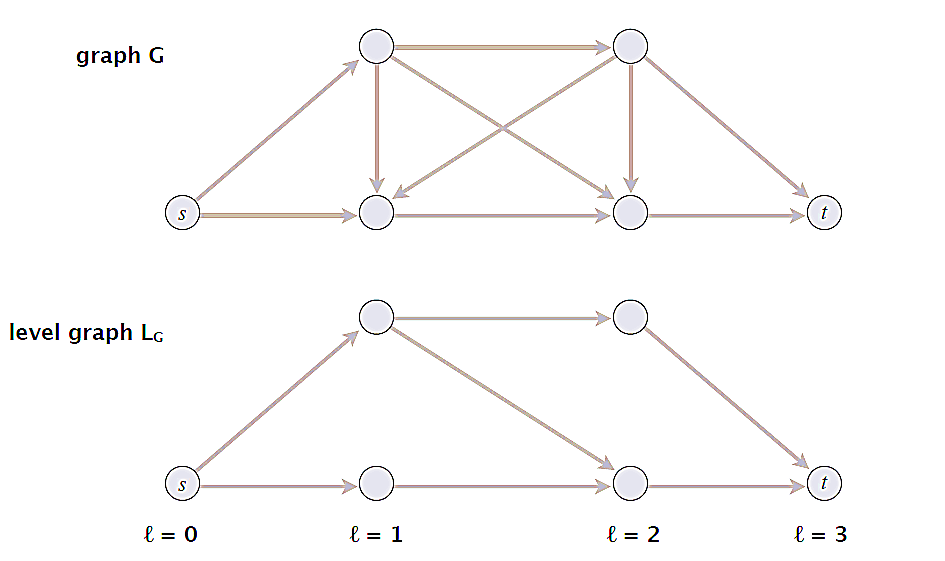
\includegraphics[width=0.7\textwidth]{figures/p50}}
	}
%%//////////////////////////////////////////////////////////////////////////////////////////////%%51
\frame{
	\frametitle{Network flow: quiz 5}
	Which edges are in the level graph of the following digraph?
	\begin{enumerate}[A.]
		\item \ccb{$D\rightarrow F$}
		\item \ccb{$E\rightarrow F$}
		\item  Both A and B.
		\item Neither A nor B.
	\end{enumerate}
	
	\vspace{1cm}\centerline{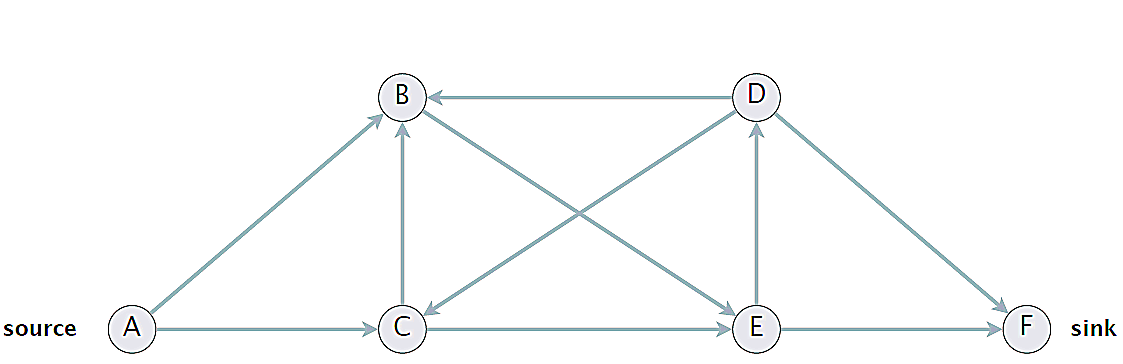
\includegraphics[width=\textwidth]{figures/p51}}
	
}


%%//////////////////////////////////////////////////////////////////////////////////////////////%%52


\frame{
	\frametitle{Shortest augmenting path: analysis}
	\begin{definition}
        Given a \ccp{digraph} \ccb{$G = (V, E)$} with source \ccb{$s$}, its \ccp{level graph} is defined by:
        \vspace{-4mm}
\begin{itemize}
	\item \ccb{$\ell(v)$ = number of edges in shortest $s\rightsquigarrow v$ path}.
	\item \ccb{$L_G = (V,E_G)$} is the subgraph of \ccb{$G$} that contains only those edges \ccb{$(v, w) \in E$}
	with  \ccb{$\ell(w) = \ell(v) + 1$}.
\end{itemize}
\end{definition}

\cco{Key property.} \ccb{$P$} is a shortest \ccb{$s\rightsquigarrow v$} path in \ccb{$G$} iff \ccb{$P$}  is an \ccb{$s\rightsquigarrow v$}  path in \ccb{$L_G$}.
	
	\vspace{1cm}\centerline{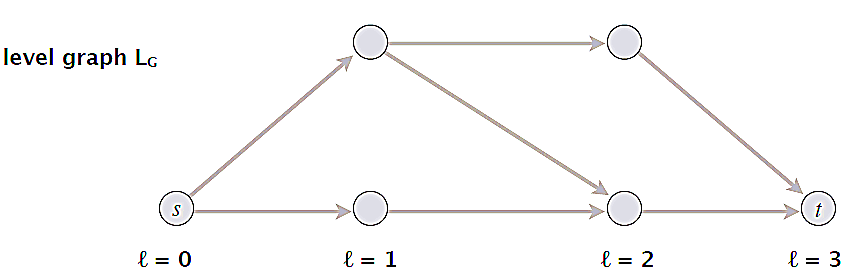
\includegraphics[width=0.8\textwidth]{figures/p52}}
}


	
	%%%%//////////////////////////////////////////////////////////////////////////////////////////////%%53
	%%
	\frame{
		\frametitle{Shortest augmenting path: analysis}
	\begin{block}{Lemma 1}
		The length of a shortest augmenting path never decreases.
	\end{block}\pause\vspace{-1em}

     \ccm{\em Proof.}\pause\vspace{-1em}
	\begin{itemize}
		\item Let \ccb{$f$} and \ccb{$f'$}  be flow before and after a shortest-path augmentation.
		\item  Let \ccb{$L_G$} and \ccb{$L_{G'}$} be level graphs of \ccb{$G_f$} and \ccb{$G_{f'}$}.
		\item Only back edges added to \ccb{$G_{f'}$} \\
		(any \ccb{$s\rightsquigarrow t$} path that uses a back edge is longer than previous length)
	\end{itemize}

    \centerline{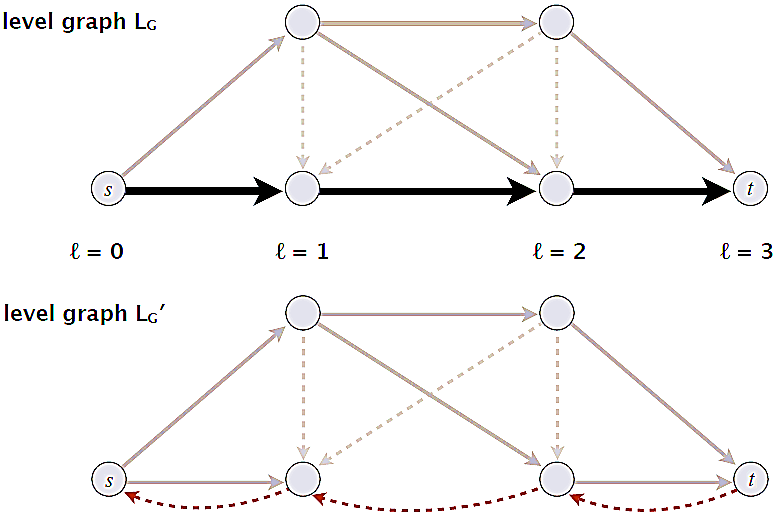
\includegraphics[width=0.6\textwidth]{figures/p53}}     	
	}
	%%%%%//////////////////////////////////////////////////////////////////////////////////////////////%%54
	%%%
	\frame{
		\frametitle{Shortest augmenting path: analysis}
	    \begin{block}{Lemma 2}
    After at most \ccb{$m$} shortest-path augmentations, the length of a shortest augmenting path strictly increases.
    \end{block}\pause\vspace{-1em}
     \ccm{\em Proof.}\pause\vspace{-1em}
	\begin{itemize}
	\item  At least one (bottleneck) edge is deleted from \ccb{$L_G$} per augmentation.
	\item No new edge added to \ccb{$L_G$} until shortest path length strictly increases.
		\end{itemize}
		
		\vspace{3mm}\centerline{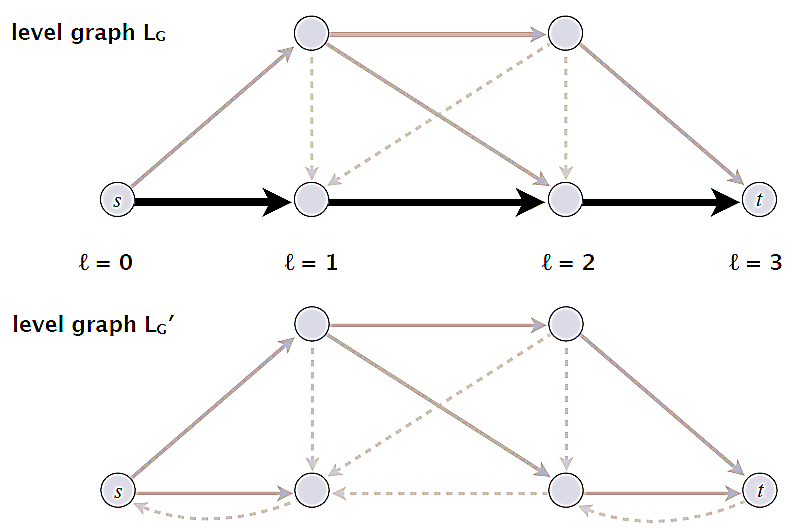
\includegraphics[width=.65\textwidth]{figures/p54}}
		
	}
	

	
	
	%%//////////////////////////////////////////////////////////////////////////////////////////////%%55
	\frame{
		\frametitle{Shortest augmenting path: review of analysis}
	\begin{block}{Lemma 1}
		The length of a shortest augmenting path never decreases.
	\end{block}

    \begin{block}{Lemma 2}
    After at most \ccb{$m$} shortest-path augmentations, the length of a shortest augmenting path strictly increases.
    \end{block}

    \begin{theorem}
    The shortest-augmenting-path algorithm takes \ccb{$O(m^2 n)$} time.
    \end{theorem}
   	
	}
	
	%%//////////////////////////////////////////////////////////////////////////////////////////////%%56
	
	\frame{
		\frametitle{Shortest augmenting path: improving the running time}
		
		
		\cco{Note.}  \ccb{$\Theta(m n)$} augmentations necessary for some flow networks.
		\pause\hspace{-2em}
		\begin{itemize}
			\item Try to decrease time per augmentation instead.
			\item Simple idea \ccc{$\Rightarrow$} \ccb{$\ccb{O(mn^2)}$}   \hspace{2em }[\ccc{Dinitz 1970}]\pause
			\item Dynamic trees \ccc{$\Rightarrow$} \ccb{$O(m n \log n)$}   \hspace{2em}  [\ccc{Sleator–Tarjan 1983}]
		\end{itemize}
	\vspace{3mm}\centerline{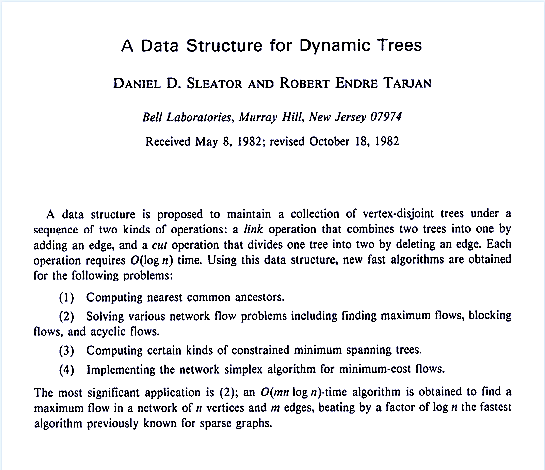
\includegraphics[width=0.8\textwidth,height=5cm]{figures/p56}}
	}

%%//////////////////////////////////////////////////////////////////////////////////////////////%%58

\section{Dinitz' Algorithm}
	
%%//////////////////////////////////////////////////////////////////////////////////////////////%%58
	
      \frame{
		\frametitle{Dinitz' algorithm}
    	\cco{Two types of augmentations.}
		\begin{itemize}\vspace{-3mm}
			\item \ccp{Normal}: length of shortest path does not change.
			\item \ccp{Special}: length of shortest path strictly increases.
		\end{itemize}\pause
		
		\ccp{Phase of normal augmentations.}
%\ccr{$\longleftarrow\begin{array}{l}{\text {\tiny within a phase, length of shortest }} \\[-2mm] {\text {\tiny augmenting path does not change %}}\end{array}$}
	\begin{itemize}\vspace{-3mm}
		\item Construct level graph \ccb{$L_G$}.
	\ccg{	\item Start at $s$, advance along an edge in $L_G$ until reach $t$ or get stuck.
	\item If reach $t$, augment flow; update $L_G$; and restart from $s$.
		\item If get stuck, delete node from $L_G$ and retreat to previous node.}
	\end{itemize}
		
	\vspace{3mm}\centerline{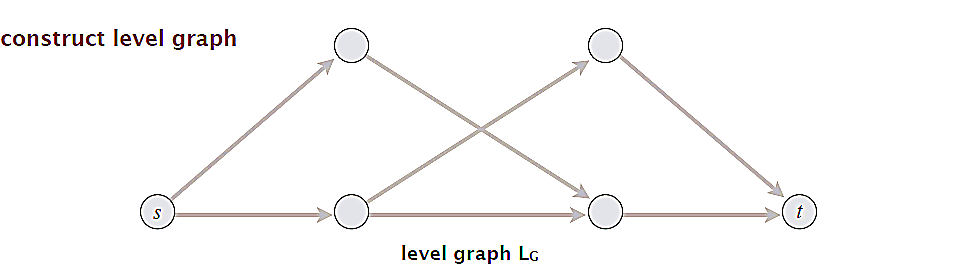
\includegraphics[width=0.8\textwidth]{figures/p58}}
	}
	
	
	
%	%%%%//////////////////////////////////////////////////////////////////////////////////////////////%%59
	
   \frame{
	\frametitle{Dinitz' algorithm}
		\cco{Two types of augmentations.}
		\begin{itemize}\vspace{-3mm}
			\item \ccp{Normal}: length of shortest path does not change.
			\item \ccp{Special}: length of shortest path strictly increases.
		\end{itemize}
	
	\ccp{Phase of normal augmentations.}
	\begin{itemize}\vspace{-3mm}
		\ccg{	\item Construct level graph $L_G$.}
		\item Start at \ccb{$s$}, advance along an edge in \ccb{$L_G$} until reach \ccb{$t$} or get stuck.
		\ccg{	\item If reach $t$, augment flow; update $L_G$; and restart from $s$.
			\item If get stuck, delete node from $L_G$ and retreat to previous node.}
	\end{itemize}
	\vspace{3mm}\centerline{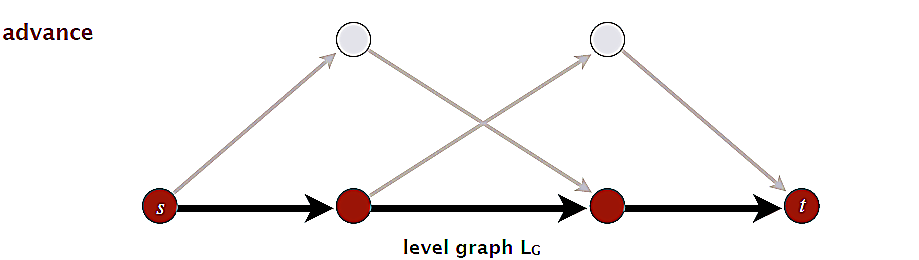
\includegraphics[width=0.73\textwidth]{figures/p59}}
	
}
%	%%%%//////////////////////////////////////////////////////////////////////////////////////////////%%60

    \frame{
	 \frametitle{Dinitz' algorithm}
		\cco{Two types of augmentations.}
		\begin{itemize}\vspace{-3mm}
			\item \ccp{Normal}: length of shortest path does not change.
			\item \ccp{Special}: length of shortest path strictly increases.
		\end{itemize}
	
	\ccp{Phase of normal augmentations.}
	\begin{itemize}\vspace{-3mm}
		\ccg{	\item Construct level graph $L_G$.
		\item Start at $s$, advance along an edge in $L_G$ until reach $t$ or get stuck.}
		\item If reach \ccb{$t$}, augment flow; update \ccb{$L_G$}; and restart from \ccb{$s$}.
		\ccg{	\item If get stuck, delete node from $L_G$ and retreat to previous node.}
	\end{itemize}
	
	\vspace{3mm}\centerline{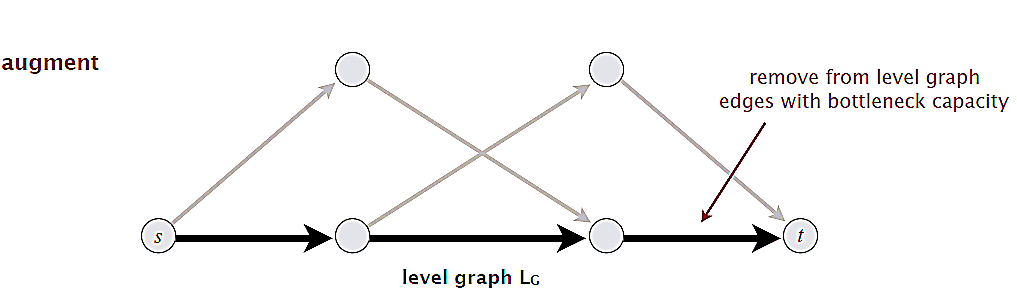
\includegraphics[width=0.8\textwidth]{figures/p60}}
}
%	%%%%//////////////////////////////////////////////////////////////////////////////////////////////%%61

   \frame{
	\frametitle{Dinitz' algorithm}
		\cco{Two types of augmentations.}
		\begin{itemize}\vspace{-3mm}
			\item \ccp{Normal}: length of shortest path does not change.
			\item \ccp{Special}: length of shortest path strictly increases.
		\end{itemize}
	
	\ccp{Phase of normal augmentations.}
	\begin{itemize}\vspace{-3mm}
	\ccg{\item Construct level graph $L_G$.}
		\item Start at \ccb{$s$}, advance along an edge in \ccb{$L_G$} until reach \ccb{$t$} or get stuck.
		\ccg{\item If reach $t$, augment flow; update $L_G$; and restart from $s$.
			\item If get stuck, delete node from {$L_G$} and retreat to previous node.}
	\end{itemize}
	\vspace{3mm}\centerline{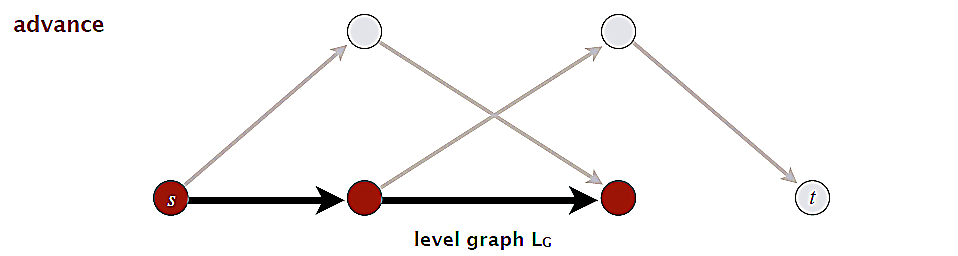
\includegraphics[width=0.8\textwidth]{figures/p61}}
	
}
%	%%%%//////////////////////////////////////////////////////////////////////////////////////////////%%62

     \frame{
  \frametitle{Dinitz' algorithm}
	
	\cco{Two types of augmentations.}
		\begin{itemize}\vspace{-3mm}
			\item \ccp{Normal}: length of shortest path does not change.
			\item \ccp{Special}: length of shortest path strictly increases.
		\end{itemize}
	
	\ccp{Phase of normal augmentations.}
	\begin{itemize}\vspace{-3mm}
		\ccg{	\item Construct level graph $L_G$.
		\item Start at $s$, advance along an edge in $L_G$ until reach $t$ or get stuck.
		\item If reach $t$, augment flow; update $L_G$; and restart from $s$.}
		\item If get stuck, delete node from \ccb{$L_G$} and retreat to previous node.
	\end{itemize}
	
	\vspace{3mm}\centerline{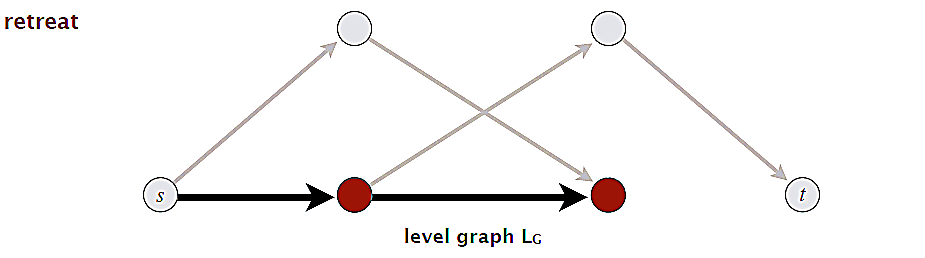
\includegraphics[width=0.8\textwidth]{figures/p62}}
}

%	%%%%//////////////////////////////////////////////////////////////////////////////////////////////%%63
\frame{
	\frametitle{Dinitz' algorithm}
		\cco{Two types of augmentations.}
		\begin{itemize}\vspace{-3mm}
			\item \ccp{Normal}: length of shortest path does not change.
			\item \ccp{Special}: length of shortest path strictly increases.
		\end{itemize}
	
	\ccp{Phase of normal augmentations.}
	\begin{itemize}\vspace{-3mm}
		\ccg{	\item Construct level graph $L_G$.}
		\item Start at \ccb{$s$}, advance along an edge in \ccb{$L_G$} until reach \ccb{$t$} or get stuck.
		\ccg{	\item If reach $t$, augment flow; update $L_G$; and restart from $s$.
		\item If get stuck, delete node from $L_G$ and retreat to previous node.}
	\end{itemize}
	
	\vspace{3mm}\centerline{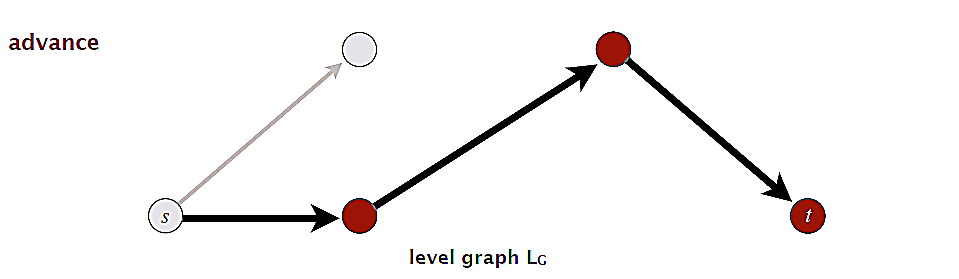
\includegraphics[width=0.8\textwidth]{figures/p63}}
}
%	%%%%//////////////////////////////////////////////////////////////////////////////////////////////%%64
    \frame{
	\frametitle{Dinitz' algorithm}
		\cco{Two types of augmentations.}
		\begin{itemize}\vspace{-3mm}
			\item \ccp{Normal}: length of shortest path does not change.
			\item \ccp{Special}: length of shortest path strictly increases.
		\end{itemize}

	
	\ccp{Phase of normal augmentations.}
	\begin{itemize}\vspace{-3mm}
		\ccg{	\item Construct level graph $L_G$.
		\item Start at $s$, advance along an edge in $L_G$ until reach $t$ or get stuck.}
			\item If reach \ccb{$t$}, augment flow; update \ccb{$L_G$}; and restart from \ccb{$s$}.
			\ccg{\item If get stuck, delete node from $L_G$ and retreat to previous node.}
	\end{itemize}
	
	\vspace{3mm}\centerline{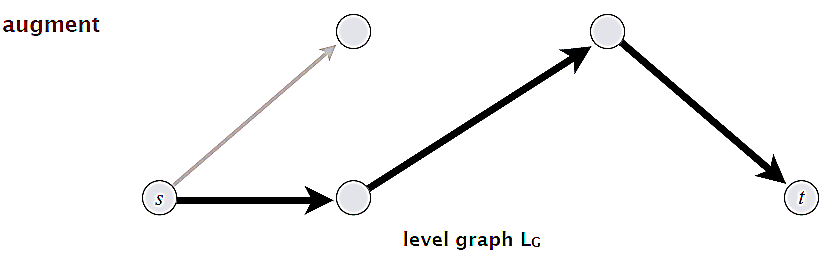
\includegraphics[width=0.7\textwidth]{figures/p64}}
}
%	%%%%//////////////////////////////////////////////////////////////////////////////////////////////%%65
\frame{
	\frametitle{Dinitz' algorithm}
		\cco{Two types of augmentations.}
		\begin{itemize}\vspace{-3mm}
			\item \ccp{Normal}: length of shortest path does not change.
			\item \ccp{Special}: length of shortest path strictly increases.
		\end{itemize}
	
	\ccb{Phase of normal augmentations.}
	\begin{itemize}\vspace{-3mm}
		\ccg{	\item Construct level graph $L_G$.}
		\item Start at \ccb{$s$}, advance along an edge in \ccb{$L_G$} until reach \ccb{$t$} or get stuck.
		\ccg{	\item If reach $t$, augment flow; update $L_G$; and restart from $s$.
			\item If get stuck, delete node from $L_G$ and retreat to previous node.}
	\end{itemize}
	
	\vspace{3mm}\centerline{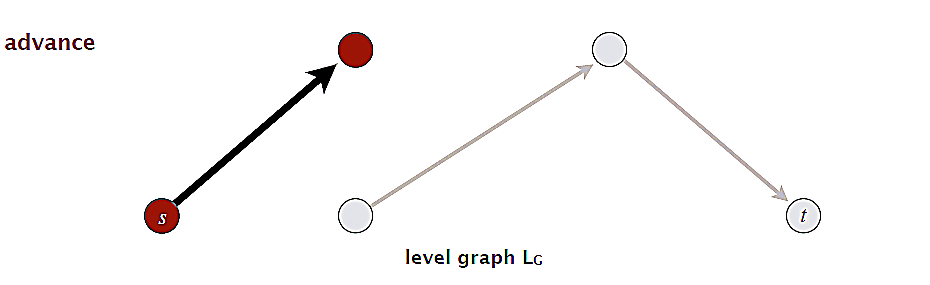
\includegraphics[width=0.8\textwidth]{figures/p65}}
}
%	%%%%//////////////////////////////////////////////////////////////////////////////////////////////%%66
\frame{
	\frametitle{Dinitz' algorithm}
		\cco{Two types of augmentations.}
		\begin{itemize}\vspace{-3mm}
			\item \ccp{Normal}: length of shortest path does not change.
			\item \ccp{Special}: length of shortest path strictly increases.
		\end{itemize}
	
	\ccb{Phase of normal augmentations.}
	\begin{itemize}\vspace{-3mm}
			\ccg{ \item Construct level graph $L_G$.
		\item Start at $s$, advance along an edge in $L_G$ until reach $t$ or get stuck.
		\item If reach $t$, augment flow; update $L_G$; and restart from $s$.}
			\item If get stuck, delete node from \ccb{$L_G$} and retreat to previous node.
	\end{itemize}
	\vspace{3mm}\centerline{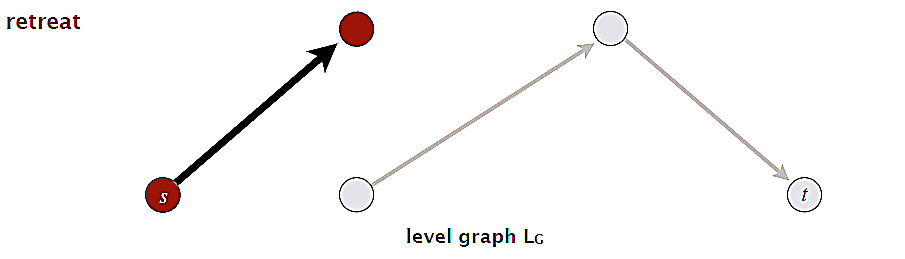
\includegraphics[width=0.8\textwidth]{figures/p66}}
	
}
%	%%%%//////////////////////////////////////////////////////////////////////////////////////////////%%67
\frame{
	\frametitle{Dinitz' algorithm}
		\cco{Two types of augmentations.}
		\begin{itemize}\vspace{-3mm}
			\item \ccp{Normal}: length of shortest path does not change.
			\item \ccp{Special}: length of shortest path strictly increases.
		\end{itemize}
	
	\ccb{Phase of normal augmentations.}
	\begin{itemize}\vspace{-3mm}
		\ccg{ \item Construct level graph $L_G$.
			\item Start at $s$, advance along an edge in $L_G$ until reach $t$ or get stuck.
			\item If reach $t$, augment flow; update $L_G$; and restart from $s$.}
		\item If get stuck, delete node from \ccb{$L_G$} and retreat to previous node.
	\end{itemize}
	
	\vspace{3mm}\centerline{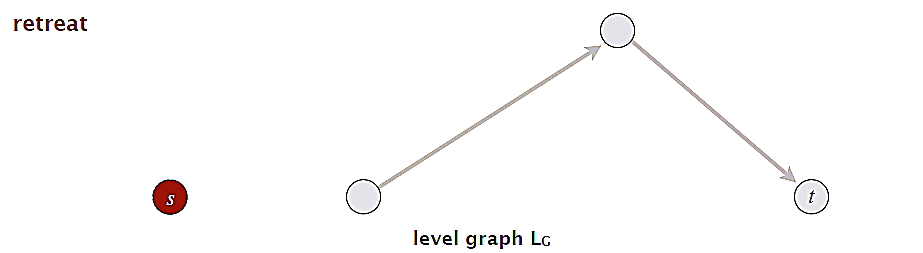
\includegraphics[width=0.8\textwidth]{figures/p67}}
}
%	%%%%//////////////////////////////////////////////////////////////////////////////////////////////%%68
\frame{
	\frametitle{Dinitz' algorithm}
	
		\cco{Two types of augmentations.}
		\begin{itemize}\vspace{-3mm}
			\item \ccp{Normal}: length of shortest path does not change.
			\item \ccp{Special}: length of shortest path strictly increases.
		\end{itemize}

	
\ccb{Phase of normal augmentations.}
\begin{itemize}\vspace{-3mm}
	\item Construct level graph $L_G$.
	\item Start at $s$, advance along an edge in $L_G$ until reach $t$ or get stuck.
	\item If reach $t$, augment flow; update $L_G$; and restart from $s$.
	\item If get stuck, delete node from $L_G$ and retreat to previous node.
\end{itemize}
\vspace{3mm}\centerline{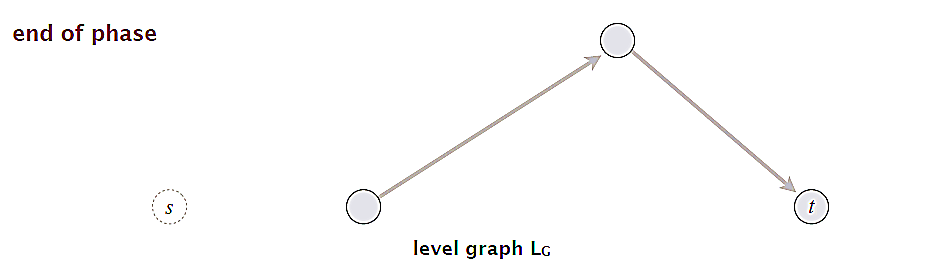
\includegraphics[width=0.8\textwidth]{figures/p68}}
}



%	%%%%//////////////////////////////////////////////////////////////////////////////////////////////%%69
	\frame{
		\frametitle{Dinitz' algorithm (as refined by Even and Itai)}

\begin{exampleblock}{}
\scalebox{.9}	{
\begin{columns}[T]
		\begin{column}{5cm}

       \begin{algorithm}[H]
        \SetKwData{x}{x}\SetKwData{y}{y}\SetKwData{z}{z}
        \SetKwFunction{Return}{\sc Return}\SetKwFunction{Init}{\sc Initialize}\SetKwFunction{Adv}{\sc Advance}
        \SetKwFunction{Up}{\sc Update}\SetKwFunction{Au}{\sc Augment}\SetKwFunction{BFS}{\sc BFS}\SetKwFunction{GT}{\sc goto}
        \SetKwInOut{Input}{input}\SetKwInOut{Output}{output}
     \Init{$G$, $f$}
     \BlankLine
     $L_{G} \leftarrow \text { level-graph of } G_{f}$\\
			$P \leftarrow \varnothing$\\
	  \GT \Adv{$s$}\;

     \end{algorithm}

     \vspace{9mm}

    \begin{algorithm}[H]
        \SetKwData{x}{x}\SetKwData{y}{y}\SetKwData{z}{z}
        \SetKwFunction{Return}{\sc Return}\SetKwFunction{Init}{\sc Initialize}\SetKwFunction{Adv}{\sc Advance}
        \SetKwFunction{Up}{\sc Update}\SetKwFunction{Au}{\sc Augment}\SetKwFunction{BFS}{\sc BFS}\SetKwFunction{GT}{\sc goto}
        \SetKwFunction{Re}{\sc Retreat}
        \SetKwInOut{Input}{input}\SetKwInOut{Output}{output}
     \Re{$v$}
     \BlankLine
      \lIf{$v=s$}{Stop}
      \Else{
      Delete $v$ from $L_G$\;
		Remove last edge $(u, v)$ from $P$\;
      }
    \GT \Adv{$u$}\;
     \end{algorithm}
		\end{column}
	
	\begin{column}{5cm}
		
 \begin{algorithm}[H]
        \SetKwData{x}{x}\SetKwData{y}{y}\SetKwData{z}{z}
        \SetKwFunction{Return}{\sc Return}\SetKwFunction{Init}{\sc Initialize}\SetKwFunction{Adv}{\sc Advance}
        \SetKwFunction{Up}{\sc Update}\SetKwFunction{Au}{\sc Augment}\SetKwFunction{BFS}{\sc BFS}\SetKwFunction{GT}{\sc goto}
        \SetKwFunction{Re}{\sc Retreat}
        \SetKwInOut{Input}{input}\SetKwInOut{Output}{output}
     \Adv{$v$}
     \BlankLine
      \If {$v=t$}{
        \Au{$P$}\;
	    Remove saturated edges from $L_G$\;
        $P\leftarrow \varnothing$\;
	    \GT  \Adv{$s$}\;
       }

      \If{there exists edge $(v, w) \in L_G$}{
	   Add edge $(v, w)$ to $P$\;
	   \GT \Adv{$w$}\;
       }
       \Else{
        \GT \Re{$v$}\;
        }
     \end{algorithm}
	\end{column}
	\end{columns}}
\end{exampleblock}		
	}

%	%%%%//////////////////////////////////////////////////////////////////////////////////////////////%%70
	\frame{
		\frametitle{Network flow: quiz 6}
		How to compute the level graph $L_G$ efficiently?
\begin{enumerate}
	\item Depth-first search.
	\item Breadth-first search.
	\item Both A and B.
	\item Neither A nor B.
\end{enumerate}

\vspace{5mm}\centerline{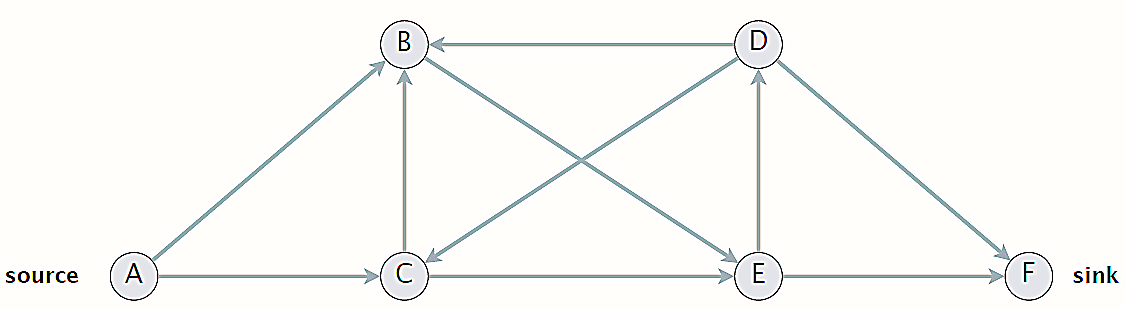
\includegraphics[width=\textwidth]{figures/p70}}
	}

%	%%%%//////////////////////////////////////////////////////////////////////////////////////////////%%71
	\frame{
		\frametitle{Dinitz' algorithm: analysis}
		\begin{lemma}
			A phase can be implemented to run in \ccb{$O(m n)$}  time.
		\end{lemma}
    \pause

	\ccm{\em Proof.}
	\begin{itemize}
		\item Initialization happens once per phase. \pause \ccpk{using BFS}\pause
		\item At most \ccb{$m$} augmentations per phase. \pause \ccpk {$\longleftarrow O(mn)$  per phase}\\\pause
		(because an augmentation deletes at least one edge from \ccb{$L_G$})\pause
		\item At most \ccb{$n$} retreats per phase.  \pause \ccpk {$\longleftarrow O(m + n)$  per phase}\\ \pause
		(because a retreat deletes one node from \ccb{$L_G$})\pause
	   \item At most \ccb{$mn$} advances per phase.  \pause \ccpk{$\longleftarrow O(mn)$  per phase}\\\pause
		(because at most \ccb{$n$} advances before retreat or augmentation)
	\end{itemize}
}

	\frame{
		\frametitle{Dinitz' algorithm: analysis}


 \begin{theorem}[Dinitz 1970]
 Dinitz' algorithm runs in \ccb{$O(mn^2)$}  time.
 \end{theorem}\pause
\ccm{\em Proof.}\pause
\begin{itemize}
	\item By Lemma, \ccb{$O(mn)$} time per phase.\pause
	\item At most \ccb{$n-1$} phases \pause (as in shortest-augmenting-path analysis).
\end{itemize}
	}
	
	
	
	
	
	%%//////////////////////////////////////////////////////////////////////////////////////////////%%72
	\frame{
		\frametitle{Augmenting-path algorithms: summary}
		\begin{table}\footnotesize
			\renewcommand{\arraystretch}{2,5}%表格行与行的距离系数
			\begin{tabular}{|c|c|c|c|}
				\hline \rowcolor{lightgray}
				year   &method& \# augmentations &running time \\
				\hline
				1955   & augmenting path & \ccb{$n C$} & \ccb{$O(m n C)$}  \\
				\hline
				1972  & fattest path &  \ccb{$m \log (m C)$} & \ccb{$O\left(m^{2} \log n \log (m C)\right)$}\\
				\hline
				1972  &capacity scaling & \ccb{$m \log C$}&  \ccb{$O\left(m^2 \log C\right)$}\\
				\hline
				1985	& improved capacity scaling &  \ccb{$m \log C$} & \ccb{$O(m n \log C)$}\\
				\hline
				1970	& shortest augmenting path & \ccb{$mn$} & \ccb{$O\left(m^{2} n\right)$} \\
				\hline
				1970	& level graph & \ccb{$mn$} &  \ccb{$O\left(m n^{2}\right)$}\\
				\hline
				1983  & dynamic trees & \ccb{$mn$} & \ccb{$ O(m n \log n)$}\\
				\hline
			\end{tabular} \\\vspace{4mm}
			{\bfseries\footnotesize augmenting-path algorithms with \ccb{$m$} edges, \ccb{$n$} nodes, and integer capacities between \ccb{1} and \ccb{$C$}}
		\end{table} 		
	}
	
	
	

	%%%%//////////////////////////////////////////////////////////////////////////////////////////////%%73
\frame{
	\frametitle{Maximum-flow algorithms: theory highlights}
	\begin{table}\scriptsize
		\renewcommand{\arraystretch}{2.0}%表格行与行的距离系数
		\begin{tabular}{|c|c|c|c|}
			\hline \rowcolor{lightgray}
			year   &method& worst case & discovered by\\
			\hline
			1951   & simplex & \ccb{$O\left(m n^{2} C\right)$} & Dantzig \\
			\hline
			1955  & augmenting paths &  \ccb{$O(m n C)$} & Ford–Fulkerson\\
			\hline
			1970 &shortest augmenting paths & \ccb{$O\left(m n^{2}\right)$} &Edmonds–Karp, Dinitz\\
			\hline
			1974	& blocking flows&  \ccb{$O\left(n^{3}\right)$} & Karzanov \\
			\hline
			1983	& dynamic trees & \ccb{$O(m n \log n)$} & Sleator–Tarjan\\
			\hline
			1985	& improved capacity scaling& \ccb{$O(m n \log C)$} &Gabow\\
			\hline
			1988  & push–relabel& \ccb{$O\left(m n \log \left(n^{2} / m\right)\right)$} & Goldberg–Tarjan\\
			\hline
			1998 & binary blocking flows & \ccb{$O\left(m^{3 / 2} \log \left(n^{2} / m\right) \log C\right)$} & Goldberg–Rao\\
			\hline
			2013 & compact networks & \ccb{$O(m n)$} &Orlin\\
			\hline
		   2014 & interior-point methods & \ccb{$\tilde{O}\left(m m^{1 / 2} \log C\right)$} & Lee–Sidford\\
		   	\hline
		   2016 & electrical flows & \ccb{$\tilde{O}\left(m^{10 / 7} C^{1 / 7}\right)$} &Madry\\
		   	\hline
		   20xx &  & ???&\\
		   \hline		
		\end{tabular} \\\vspace{4mm}
		{\bfseries\footnotesize augmenting-path algorithms with \ccb{$m$} edges, \ccb{$n$} nodes, and integer capacities between \ccb{1} and \ccb{$C$}}
	\end{table} 		
}


%%	%%%%//////////////////////////////////////////////////////////////////////////////////////////////%%74
%	  \frame{
%		\frametitle{Maximum-flow algorithms: practice}
%		
%		\cco{Push–relabel algorithm (Section 7.4)}. [Goldberg–Tarjan 1988]\\
%		Increases flow one edge at a time instead of one augmenting path at a time.
%		
%		\vspace{3mm}\centerline{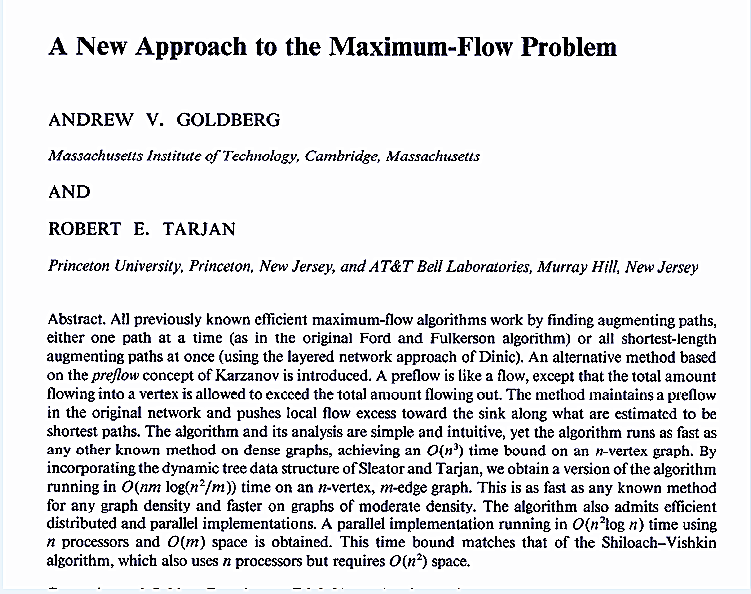
\includegraphics[width=0.8\textwidth]{figures/p74}}
%	}
%
%%	%%%%//////////////////////////////////////////////////////////////////////////////////////////////%%75
%\frame{
%	\frametitle{Maximum-flow algorithms: practice}
%	
%\cco{Caveat.}  Worst-case running time is generally not useful for predicting or comparing max-flow algorithm performance in practice.
%
%
%\cco{Best in practice.} Push–relabel method with gap relabeling: \ccb{$O(m^{3/2})$}  in practice.\vspace{6mm}
%	
%\vspace{5mm}\centerline{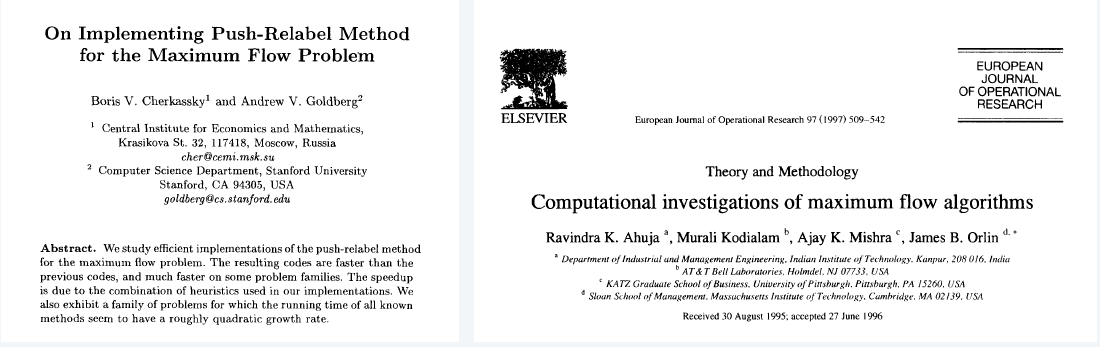
\includegraphics[width=\textwidth]{figures/p75}}
%}
%%	%%%%//////////////////////////////////////////////////////////////////////////////////////////////%%76
%\frame{
%	\frametitle{Maximum-flow algorithms: practice}
%	
%\cco{Computer vision.}  Different algorithms work better for some dense problems that arise in applications to computer vision.
%
%	\vspace{6mm}\centerline{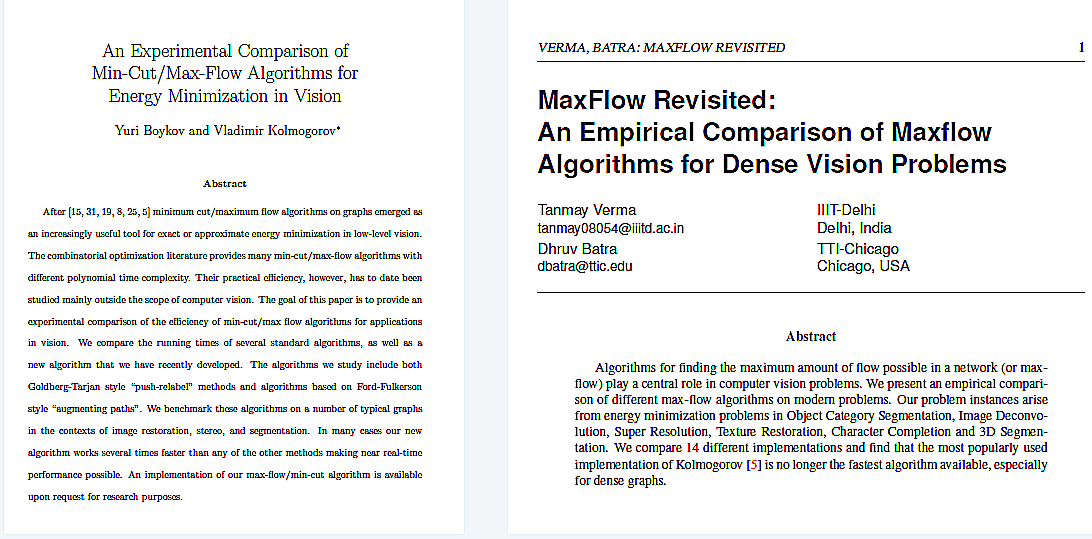
\includegraphics[width=\textwidth]{figures/p76}}
%}
%%	%%%%//////////////////////////////////////////////////////////////////////////////////////////////%%77
%
%   \frame{
%	\frametitle{Maximum-flow algorithms: Matlab}
%	\vspace{3mm}\centerline{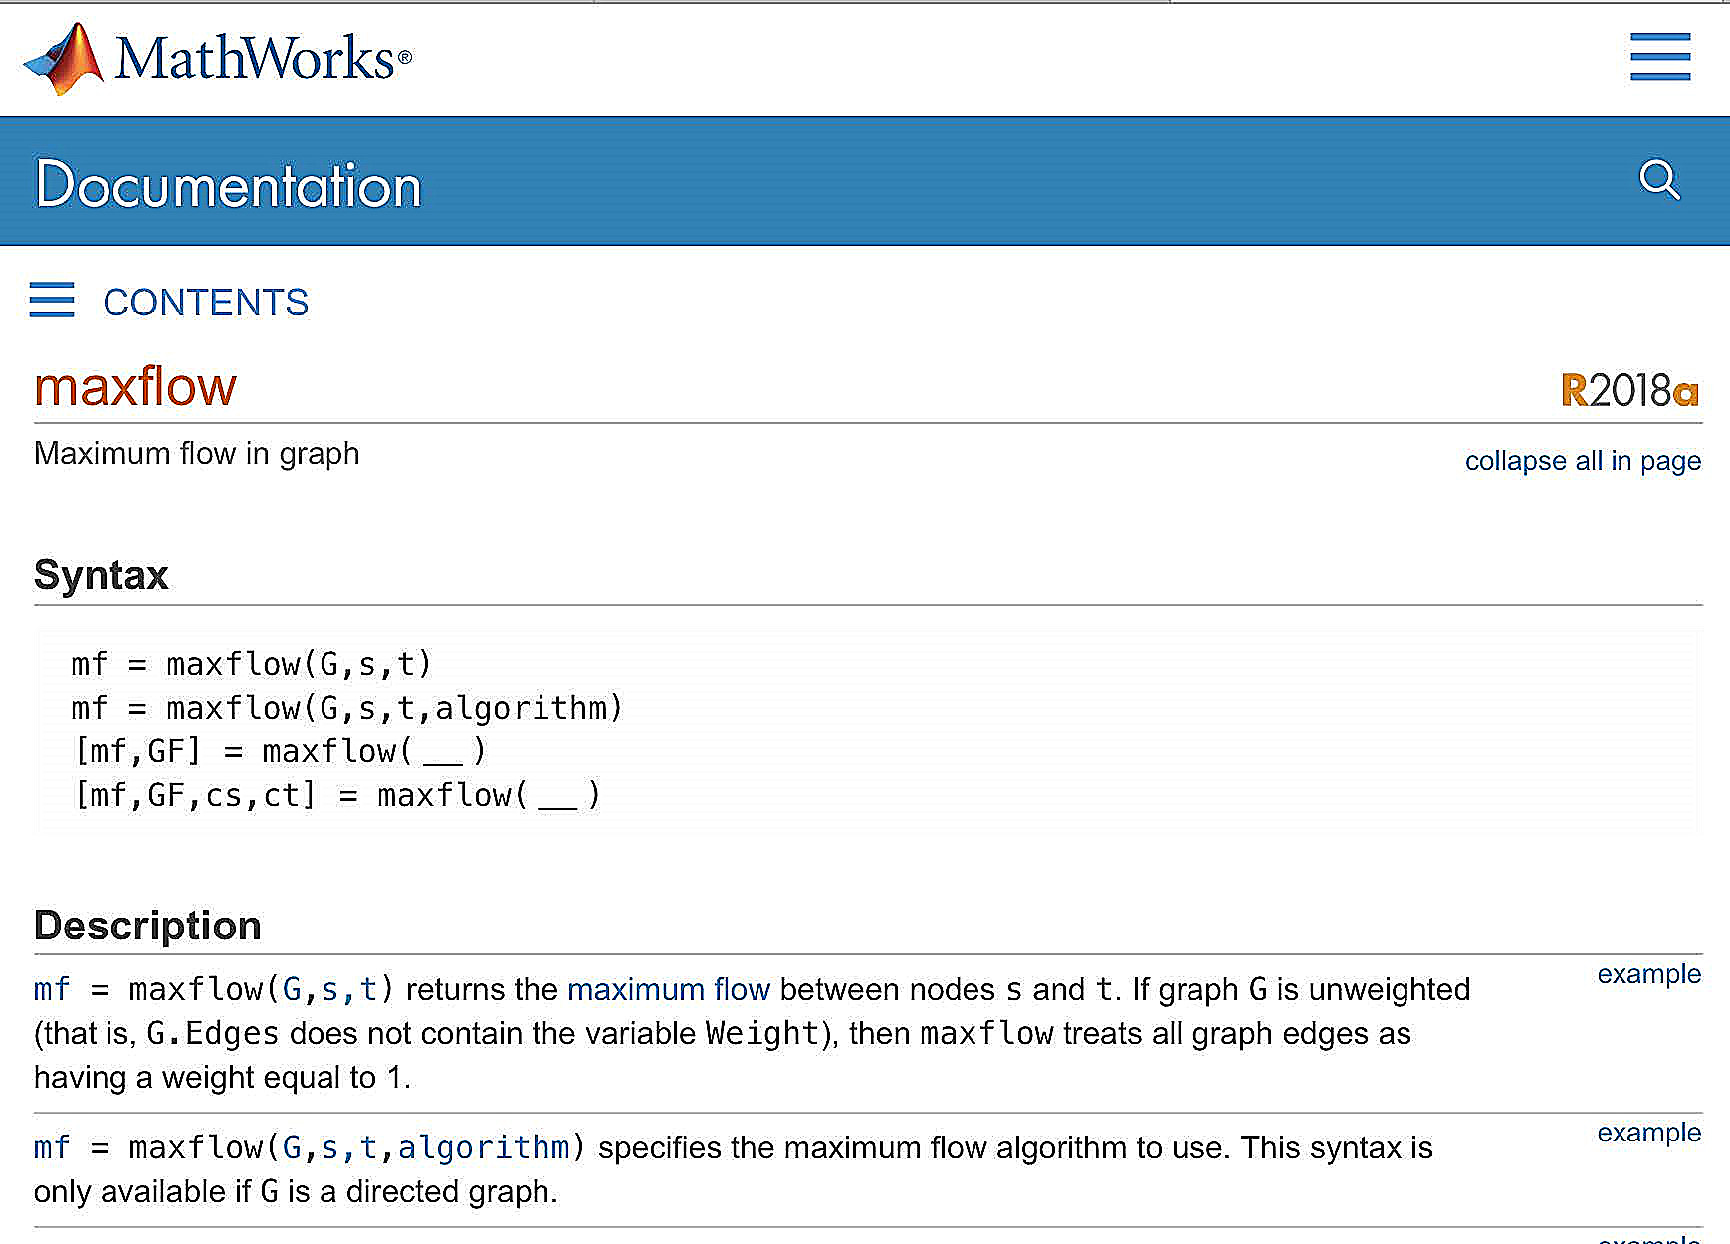
\includegraphics[width=\textwidth]{figures/p77}}
%
%}
%%	%%%%//////////////////////////////////////////////////////////////////////////////////////////////%%78
%
%	  \frame{
%		\frametitle{Maximum-flow algorithms: Google}
%		
%		\vspace{3mm}\centerline{\includegraphics[width=\textwidth]{figures/p78}}
%		
%}
%
%\section{Simple Unit-Capacity Networks}
%
%%	%%%%//////////////////////////////////////////////////////////////////////////////////////////////%%80
%	
%	
%	\frame{
%		\frametitle{Network flow: quiz 7}
%	Which max-flow algorithm to use for bipartite matching?
%	\begin{enumerate}
%		\item Ford–Fulkerson: \ccb{$O(m n C)$}.
%		\item Capacity scaling: \ccb{$O\left(m^{2} \log C\right)$}.
%		\item Shortest augmenting path: \ccb{$O\left(m^{2} n\right)$}.
%		\item Dinitz' algorithm: \ccb{$O\left(m n^{2}\right)$}.
%	\end{enumerate}
%	}
%
%%%%%//////////////////////////////////////////////////////////////////////////////////////////////%%81
%
%	\frame{
%     \frametitle{Simple unit-capacity networks}
%    \begin{definition}
%    A  flow network is a \ccp{simple unit-capacity network} if:
%    \begin{itemize}
%	\item Every edge has capacity \ccb{1}.
%	\item Every node (other than \ccb{$s$} or \ccb{$t$}) has exactly one entering edge,\\
%	or exactly one leaving edge, or both.
%    \end{itemize}
%    \end{definition}\vspace{-3mm}
%
%    }
%
%%%%%//////////////////////////////////////////////////////////////////////////////////////////////%%81
%
%	\frame{
%     \frametitle{Simple unit-capacity networks}
%       \cco{Property.}  Let \ccb{$G$} be a simple unit-capacity network and let \ccb{$f$} be a 0–1 flow. Then, residual network \ccb{$G_f$} is also a simple unit-capacity network.\pause
%
%
%    \ccc{Exercise.}  Bipartite matching.\pause
%
%    \vspace{3mm}\centerline{\includegraphics[width=0.8\textwidth,height=4cm]{figures/p81}}
%	}
%	
%%	%%%%//////////////////////////////////////////////////////////////////////////////////////////////%%82
%	\frame{
%		\frametitle{Simple unit-capacity networks}
%\cco{Shortest-augmenting-path algorithm.}\vspace{-3mm}
%\begin{itemize}
%	\item \ccp{Normal augmentation}: length of shortest path does not change.
%	\item \ccp{Special augmentation}: length of shortest path strictly increases.
%\end{itemize}\vspace{-3mm}
%	\begin{theorem}[Even–Tarjan 1975]
%	In simple unit-capacity networks, Dinitz'algorithm computes a maximum flow in \ccb{$O(m n^{1/2})$} time.
%	\end{theorem}\pause
%
%\ccm{\em Proof.}\pause
%\begin{itemize}
%	\item  \ccc{Lemma 1.} Each phase of normal augmentations takes \ccb{$O(m)$} time.
%	\item  \ccc{Lemma 2.} After \ccb{$n^{1/2}$} phases, \ccb{${val}(f) \geq {val}\left(f^{*}\right)-n^{1 / 2}$}.
%	\item  \ccc{Lemma 3.}  After \ccb{$\leq n^{1/2}$} additional augmentations, flow is optimal.
%\end{itemize}
%}
%
%%	%%%%//////////////////////////////////////////////////////////////////////////////////////////////%%82
%	\frame{
%		\frametitle{Simple unit-capacity networks}
%
%     \begin{block}{Lemma 3}
%    	After \ccb{$\leq n^{1/2}$}  additional augmentations, flow is optimal.
%	 \end{block}\pause
%
%     \ccm{\em Proof.} Each augmentation increases flow value by at least 1.
%
%    }
%
%%	%%%%//////////////////////////////////////////////////////////////////////////////////////////////%%83
%	
%	\frame{
%		\frametitle{Simple unit-capacity networks}
%\ccp{Phase of normal augmentations.}%\Ccr{$\Longleftarrow\Begin{Array}{L}{\Tiny\Text { Within A Phase, Length Of Shortest}} \\[-2Mm] {\Tiny\Text { Augmenting Path Does Not Change }}\End{Array}$}
%  \begin{itemize}\vspace{-3mm}
%	\item 	Construct level graph \ccb{$L_G$}.
%\ccg{	\item  Start at $s$, advance along an edge in $L_G$ until reach $t$ or get stuck.
%	\item  If reach $t$, augment flow; update $L_G$; and restart from $s$.
%	\item If get stuck, delete node from $L_G$ and go to previous node.}
%\end{itemize}
%
%\vspace{5mm}\centerline{\includegraphics[width=.8\textwidth]{figures/p83}}
%	}
%
%
%%	%%%%//////////////////////////////////////////////////////////////////////////////////////////////%%84
%
%\frame{
%	\frametitle{Simple unit-capacity networks}
%	\ccp{Phase of normal augmentations.}
%	\begin{itemize}\vspace{-3mm}
%		\ccg{	\item 	Construct level graph $L_G$}.
%	\item  Start at \ccb{$s$}, advance along an edge in \ccb{$L_G$} until reach \ccb{$t$} or get stuck.
%		\ccg{	\item  If reach $t$, augment flow; update $L_G$; and restart from $s$.
%		\item If get stuck, delete node from $L_G$ and go to previous node.}
%	\end{itemize}
%	
%	\vspace{5mm}\centerline{\includegraphics[width=0.8\textwidth]{figures/p84}}
%}
%
%
%
%%	%%
%%	%%%%//////////////////////////////////////////////////////////////////////////////////////////////%%85
%   \frame{
%	\frametitle{Simple unit-capacity networks}
%	\ccp{Phase of normal augmentations.}
%	\begin{itemize}\vspace{-3mm}
%		\ccg{	\item 	Construct level graph $L_G$.
%		\item  Start at $s$, advance along an edge in $L_G$ until reach $t$ or get stuck.}
%		\item  If reach \ccb{$t$}, augment flow; update \ccb{$L_G$}; and restart from \ccb{$s$}.
%		\ccg{		\item If get stuck, delete node from $L_G$ and go to previous node.}
%	\end{itemize}
%	\vspace{5mm}\centerline{\includegraphics[width=0.8\textwidth]{figures/p85}}
%	
%}
%%	%%%%//////////////////////////////////////////////////////////////////////////////////////////////%%86
%
%\frame{
%	\frametitle{Simple unit-capacity networks}
%	\ccp{Phase of normal augmentations.}
%	\begin{itemize}\vspace{-3mm}
%		\ccg{	\item 	Construct level graph $L_G$}.
%		\item  Start at \ccb{$s$}, advance along an edge in \ccb{$L_G$} until reach \ccb{$t$} or get stuck.
%		\ccg{	\item  If reach $t$, augment flow; update $L_G$; and restart from $s$.
%			\item If get stuck, delete node from $L_G$ and go to previous node.}
%	\end{itemize}
%	
%	\vspace{5mm}\centerline{\includegraphics[width=0.8\textwidth]{figures/p86}}
%}
%
%
%%	%%%%//////////////////////////////////////////////////////////////////////////////////////////////%%87
%
%\frame{
%	\frametitle{Simple unit-capacity networks}
%	\ccp{Phase of normal augmentations.}
%	\begin{itemize}\vspace{-3mm}
%		\ccg{	\item 	Construct level graph $L_G$.
%		\item  Start at $s$, advance along an edge in $L_G$ until reach $t$ or get stuck.
%		\item  If reach $t$, augment flow; update $L_G$; and restart from $s$.}
%			\item If get stuck, delete node from \ccb{$L_G$} and go to previous node.
%	\end{itemize}
%	
%	\vspace{5mm}\centerline{\includegraphics[width=0.8\textwidth]{figures/p87}}
%}
%
%%	%%%%//////////////////////////////////////////////////////////////////////////////////////////////%%88
%
%\frame{
%	\frametitle{Simple unit-capacity networks}
%	\ccp{Phase of normal augmentations.}
%	\begin{itemize}\vspace{-3mm}
%		\ccg{	\item 	Construct level graph $L_G$.}
%			\item  Start at \ccb{$s$}, advance along an edge in \ccb{$L_G$} until reach \ccb{$t$} or get stuck.
%		\ccg{	\item  If reach $t$, augment flow; update $L_G$; and restart from $s$.
%		\item If get stuck, delete node from $L_G$ and go to previous node.}
%	\end{itemize}
%	
%	\vspace{5mm}\centerline{\includegraphics[width=0.8\textwidth]{figures/p88}}
%}
%
%%	%%%%//////////////////////////////////////////////////////////////////////////////////////////////%%89
%
%\frame{
%	\frametitle{Simple unit-capacity networks}
%	\ccp{Phase of normal augmentations.}
%	\begin{itemize}\vspace{-3mm}
%		\ccg{	\item 	Construct level graph $L_G$.
%		\item  Start at $s$, advance along an edge in $L_G$ until reach $t$ or get stuck.}
%	\item  If reach \ccb{$t$}, augment flow; update \ccb{$L_G$}; and restart from \ccb{$s$}.
%			\ccg{		\item If get stuck, delete node from $L_G$ and go to previous node.}
%	\end{itemize}
%	
%	\vspace{5mm}\centerline{\includegraphics[width=0.8\textwidth]{figures/p89}}
%}
%
%
%%	%%%%//////////////////////////////////////////////////////////////////////////////////////////////%%90
%
%\frame{
%	\frametitle{Simple unit-capacity networks}
%	\ccp{Phase of normal augmentations.}
%	\begin{itemize}\vspace{-3mm}
%		\item 	Construct level graph \ccb{$L_G$}.
%			\item  Start at \ccb{$s$}, advance along an edge in \ccb{$L_G$} until reach \ccb{$t$} or get stuck.
%		\item  If reach \ccb{$t$}, augment flow; update \ccb{$L_G$}; and restart from \ccb{$s$}.
%		\item If get stuck, delete node from \ccb{$L_G$} and go to previous node.
%	\end{itemize}
%	
%	\vspace{7mm}\centerline{\includegraphics[width=.8\textwidth]{figures/p90}}
%}
%
%%	%%%%//////////////////////////////////////////////////////////////////////////////////////////////%%91
%
%\frame{
%	\frametitle{Simple unit-capacity networks}
%	\ccp{Phase of normal augmentations.}
%	\begin{itemize}\vspace{-3mm}
%		\item 	Construct level graph \ccb{$L_G$}.
%			\item  Start at \ccb{$s$}, advance along an edge in \ccb{$L_G$} until reach \ccb{$t$} or get stuck.
%		\item  If reach \ccb{$t$}, augment flow; update \ccb{$L_G$}; and restart from \ccb{$s$}.
%		\item If get stuck, delete node from \ccb{$L_G$} and go to previous node.
%	\end{itemize}
%
%
%\begin{block}{Lemma 1}
%	 A phase of normal augmentations takes \ccb{$O(m)$} time.
% \end{block}\pause
%
%\ccm{\em Proof.}\vspace{-3mm}
%\begin{itemize}
%	\item \ccb{$O(m)$} to create level graph \ccb{$L_G$}.
%	\item \ccb{$O(1)$} per edge (each edge involved in at most one advance, retreat, and\\
%	augmentation).
%	\item \ccb{$O(1)$} per node (each node deleted at most once)
%\end{itemize}
%	
%}
%%	%%%%//////////////////////////////////////////////////////////////////////////////////////////////%%92
%
%\frame{
%	\frametitle{Network flow: quiz 8}
%	Consider running advance–retreat algorithm in a unit-capacity network (but not necessarily a simple one). What is running time?\\
%\pause	\hspace{3cm}\ccr{ $ \begin{array}{l}
%		\nwarrow\\[-2mm]
%		\tiny\text{both indegree and outdegree}\\[-2mm]
%		\tiny\text{of a node can be larger than 1}
%		\end{array} $}
%\begin{enumerate}
%	\item \ccb{$O(m)$}.
%	\item \ccb{$O\left(m^{3 / 2}\right)$}.
%	\item \ccb{$O(m n)$}.
%	\item May not terminate.
%\end{enumerate}
%	
%}
%
%%	%%%%//////////////////////////////////////////////////////////////////////////////////////////////%%93
%\frame{
%	\frametitle{Computational geometry applications}
%
%	\begin{block}{Lemma 2}
%	After \ccb{$n^{1/2}$} phases, \ccb{$val( f ) \geq val( f^*) -n^{1/2}$}.
%		\end{block}\pause
%\ccm{\em Proof.}\pause
%	\begin{itemize}\vspace{-3mm}
%        \item After \ccb{$n^{1/2}$} phases, length of shortest augmenting path is \ccb{$>n^{1/2}$}.\pause
%		\item Thus, level graph has \ccb{$\geq n^{1/2}$} levels (not including levels for \ccb{$s$} or \ccb{$t$})\pause
%		\item Let \ccb{$1 \leq h \leq n^{1 / 2}$} be a level with min number of nodes \ccc{$\Rightarrow$} \ccb{$\left|V_{h}\right| \leq n^{1 / 2}$}.\pause
%	\end{itemize}
%\vspace{5mm}\centerline{\includegraphics[width=0.8\textwidth]{figures/p93}}
%}
%
%
%%	%%%%//////////////////////////////////////////////////////////////////////////////////////////////%%94
%	\frame{
%		\vspace{3mm}
%		\frametitle{Computational geometry applications}
%	\begin{block}{Lemma 2}
%	After \ccb{$n^{1/2}$} phases, \ccb{$val( f ) \geq val( f^*) -n^{1/2}$}.
%		\end{block}\vspace{-1em}
%\ccm{\em Proof.}
%	\begin{itemize}\vspace{-3mm}
%		\item After \ccb{$n^{1/2}$} phases, length of shortest augmenting path is \ccb{$>n^{1/2}$}.
%		\item Thus, level graph has \ccb{$\geq n^{1/2}$} levels (not including levels for \ccb{$s$} or \ccb{$t$})
%		\item Let \ccb{$1 \leq h \leq n^{1 / 2}$} be a level with min number of nodes \ccc{$\Rightarrow$} \ccb{$\left|V_{h}\right| \leq n^{1 / 2}$}.
%		\item Let \ccb{$A=\{v : \ell(v)<h\} \cup\{v : \ell(v)=h \text { and } v \text { has } \leq 1 $  outgoing residual edge\}} .
%		\item \ccb{$\operatorname{cap}_{f}(A, B) \leq\left|V_{h}\right| \leq n^{1 / 2} \Rightarrow \operatorname{val}(f) \geq \operatorname{val}\left(f^{*}\right)-n^{1 / 2}$}
%	\end{itemize}
%     \centerline{\includegraphics[width=0.8\textwidth]{figures/p94}}
%	}
%%	%%%%//////////////////////////////////////////////////////////////////////////////////////////////%%95
%\frame{
%\frametitle{Simple unit-capacity networks: review
%}
%\begin{theorem} [Even–Tarjan 1975]
%	In simple unit-capacity networks, Dinitz' algorithm computes a maximum flow in \ccb{$O(m n^{1/2})$} time.
%	
%\end{theorem}
%	\ccm{\em Proof.}
%	\begin{itemize}\vspace{-3mm}
%		\item Lemma 1. Each phase take \ccb{$O(m)$} time.
%		\item Lemma 2. After \ccb{$n^{1/2}$} phase, \ccb{$\operatorname{val}(f) \geq \operatorname{val}\left(f^{\prime}\right)-n^{1 / 2}$}
%		\item Lemma 3. After \ccb{$\leq n^{1/2}$} additional augmentations
%	\end{itemize}\pause
%
%\begin{corollary}
%	Dinitz' algorithm computes \ccp{max-cardinality bipartite matching} in \ccb{$O(m n^{1/2})$} time.
%\end{corollary}
%}	
\cite{algo-design}
\bibliographystyle{alpha}

\bibliography{netflow}
\end{document}
